\documentclass[a4paper,12pt]{article}
\usepackage[ansinew]{inputenc}
\usepackage[german]{babel}
\usepackage[T1]{fontenc} %Umlaute
\usepackage{lmodern}
\usepackage[top=2cm, left=2cm, bottom=2cm, right=2cm]{geometry}
\usepackage{fancybox, graphicx}
\usepackage{float}
\usepackage{listings} 
\usepackage{multirow}
\usepackage{multicol}
\usepackage{color}		 % f�r Farben im allgemeinen
\usepackage{colortbl}
\usepackage{cite}
\usepackage{bibgerm}
\usepackage{palatino}
\usepackage{chngpage}
\usepackage{chngcntr}
\usepackage{amsmath}
\usepackage{setspace}
\usepackage{subcaption}
\counterwithout{figure}{chapter}
\counterwithout{table}{chapter}
\renewcommand{\floatpagefraction}{0.85}


\usepackage{fancyhdr}
\pagestyle{fancy}

\definecolor{rot}{rgb}{1,0.3,0}
\definecolor{gelb}{rgb}{1,1,0}
\definecolor{gruen}{rgb}{0,1,0.4}


\fancyhf{}
\fancyhead[RE]{\slshape \nouppercase{\leftmark}}    % Even page header: "page   chapter"
\fancyhead[LO]{\slshape \nouppercase{\rightmark}}   % Odd  page header: "section   page"
\fancyhead[RO,LE]{\bfseries \thepage} 
\renewcommand{\headrulewidth}{1pt}    % Underline headers
\renewcommand{\footrulewidth}{0pt}    

\fancypagestyle{plain}{               % No chapter+section on chapter start pages
\fancyhf{}
\fancyhead[RO,LE]{\bfseries \thepage}
\renewcommand{\headrulewidth}{1pt}
\renewcommand{\footrulewidth}{0pt}
}

% Left headings: "1  INTRODUCTION"
%\renewcommand{\chaptermark}[1]{%
%\markboth{\thechapter\ \ \ \ #1}{}}

% Right headings: "1.1  Basics"
\renewcommand{\sectionmark}[1]{%
\markright{\thesection\ \ \ \ #1}{}}

%\lstset{language=java} 
\lstset{basicstyle=\scriptsize}
\lstset{numbers=left, numberstyle=\tiny, numbersep=2pt, breaklines=true} 
\lstset{ numberbychapter=false}
\graphicspath{{pics/}}
\newcommand{\listoflolentryname}{\lstlistingname} 
\usepackage{float}
%\newcommand{\fullcite}{\citep} %for "Author [1980]"
\usepackage[pdftex,plainpages=false,pdfpagelabels]{hyperref}
\usepackage[nonumberlist]{glossaries}

\makeglossaries
\loadglsentries{glossary}

% --- Farbdefinitionen ----------------------------------------
\definecolor{rot}{rgb}{1,0.3,0}
\definecolor{gelb}{rgb}{1,1,0}
\definecolor{gruen}{rgb}{0,1,0.4}
\definecolor{darkblue}{rgb}{0.2,0.3,1}
\definecolor{lightblue}{rgb}{0.6,0.7,1}
\definecolor{white}{rgb}{1,1,1}
\definecolor{pblue}{rgb}{0.13,0.13,1}
\definecolor{pgreen}{rgb}{0,0.5,0}
\definecolor{pred}{rgb}{0.9,0,0}
\definecolor{pgrey}{rgb}{0.46,0.45,0.48}

\onehalfspacing
\linespread{1.5}

\bibliographystyle{geralpha}

\renewcommand{\floatpagefraction}{0.85}

\usepackage[figuresright]{rotating}
\usepackage{geometry}
\geometry{a4paper,left=20mm,right=20mm} 

\newlength{\fullwidth} % Width of text plus margin notes
\setlength{\fullwidth}{\textwidth}


\lstset{language=Java,
  showspaces=false,
  showtabs=false,
  breaklines=true,
  showstringspaces=false,
  breakatwhitespace=true,
  commentstyle=\color{pgreen},
  keywordstyle=\color{pblue},
  stringstyle=\color{pred},
  basicstyle=\fontsize{9}{10}\selectfont\ttfamily,
  moredelim=[il][\textcolor{pgrey}]{$ $},
  moredelim=[is][\textcolor{pgrey}]{\%\%}{\%\%}
}


\usepackage{varwidth}
\newcommand\tabrotate[1]{\begin{turn}{90}\rlap{#1}\end{turn}}
\newcommand\tabvarwidth[2][3cm]{\begin{varwidth}[b]{#1}\centering #2\end{varwidth}}
\newcommand{\myparagraph}[1]{\paragraph{#1}\mbox{}\\}

%----------------------------------------------------------------------------------
% \vft		{ NUMBER }
%			{ UPPER_LEFT }
%			{ UPPER_RIGHT }
%			{ LOWER_LEFT }
%			{ LOWER_RIGHT }
%			{ CAPTION }
%			{ LABEL }
%
% Gleichung, die ein Matching darstellt
\newcommand{\vft}[7]{
\begin{table}[H]
\centering
\small
\doublespacing
\begin{tabular}[c]{|c|c|c|}
\hline
#1 & \cellcolor{gruen}\textbf{positiv} & \cellcolor{rot}\textbf{negativ} \\
\hline
\cellcolor{rot}&\cellcolor{rot}&\cellcolor{rot}\\
\tabrotate{\cellcolor{rot}\textbf{falsch}} & \multirow{-2}{*}{\cellcolor{rot}#2}&\multirow{-2}{*}{\cellcolor{rot}#3}\\
\hline
\cellcolor{gruen}&\cellcolor{gruen}&\cellcolor{rot}\\
\tabrotate{\cellcolor{gruen}richtig} &\multirow{-2}{*}{\cellcolor{gruen}#4}&\multirow{-2}{*}{\cellcolor{rot}#5} \\
\hline
\end{tabular}
\singlespacing
\caption{#6}
 \label{tab:#7}
\end{table}
}
%----------------------------------------------------------------------------------
% \matchTyp		{ LEFT }
%				{ MATCHERVAR }
%				{ RIGHT }
%
% Gleichung, die ein Matching darstellt
\newcommand{\matchTyp}[3]
{
#1 \equiv_{#2} #3
}

%----------------------------------------------------------------------------------
% \inhTyp		{ CHILD }
%				{ PARENT }
%
% Gleichung, die eine Vererbung darstellt
\newcommand{\inhTyp}[2]
{
#1 \leq #2
}

%----------------------------------------------------------------------------------
% \selTyp		{ WRAPPER }
%				{ ATTR }
%
% Gleichung, die eine Selektion darstellt
\newcommand{\selTyp}[2]
{
#1 \# #2
}

%----------------------------------------------------------------------------------
% \delegate		{ SOURCE }
%				{ TARGET }
%
% Gleichung, die eine Delegation darstellt
\newcommand{\delegate}[2]
{
#1 \Rightarrow #2
}

%----------------------------------------------------------------------------------
% \applyMatcher		{ MATCHER }
%					{ PARAM }
%
% Gleichung, die Applikation eines Matchers auf einen Parameter 
\newcommand{\applyMatcher}[2]
{
(#1)#2
}

%----------------------------------------------------------------------------------
% matcherEquivDef		{ MATCHER }
%						
%
% Umgebung f�r die Definition der �bereinstimmung eines Matchers
\newenvironment{matcherEquivDef}[1]{
\begin{addmargin}[1in]{0cm}
\underline{�bereinstimmung (#1)}
\end{addmargin}
\begin{eqnarray*}
}
{
\end{eqnarray*}
}

%----------------------------------------------------------------------------------
% matcherConvDef		{ MATCHER }
%						{ ANNAHME }
%
% Umgebung f�r die Definition der �bereinstimmung eines Matchers
\newenvironment{matcherConvDef}[2]{
\begin{addmargin}[1in]{0cm}
\underline{Konvertierung (#1)}\newline
#2
\end{addmargin}
\begin{eqnarray*}
}
{
\end{eqnarray*}
}

%----------------------------------------------------------------------------------
% \myFigure	[ LABEL_PREFIX (optional) ]
%				{ FILENAME (without extension) }
%				{ CAPTION TEXT }
%				{ SHORT VERSION OF CAPTION TEXT }
%
%Bild wird in Originalgroesse gesetzt
%picture using full width of the page
\newcommand{\myFigure}[3]
{
\begin{figure}[H]
	\center{
	\begin{minipage}{\fullwidth}
	\center{
		\includegraphics{#1}
		\caption{#2}
		\label{abb:#3}
		}
	\end{minipage}
	}
\end{figure}
}

%----------------------------------------------------------------------------------
% \myBigFigure	[ WIDTH (optional) ]
%				{ FILENAME (without extension) }
%				{ CAPTION TEXT }
%				{ SHORT VERSION OF CAPTION TEXT }
%
%Bild wird in kompletter Breite gesetzt
%picture using full width of the page
\newcommand{\myBigFigure}[4][\fullwidth]
{
\begin{figure}[H]
	\center{
	\begin{minipage}{#1}
		\includegraphics[width=#1]{#2}
		\caption{#3}
		\label{abb:#4}
	\end{minipage}
	}
\end{figure}
}


%----------------------------------------------------------------------------------
% \myBigFigureGraphic	
%						[ PARAMS (optional) ]
%				{ FILENAME (without extension) }
%				{ CAPTION TEXT }
%				{ SHORT VERSION OF CAPTION TEXT }
%
%Bild wird in kompletter Breite gesetzt
%picture using full width of the page
\newcommand{\myBigFigureGraphic}[5][width=\fullwidth]
{
\begin{figure}[H]
	\center
	\includegraphics[#1]{#2}
	\caption{#3}
	\label{abb:#4}
\end{figure}
}



%----------------------------------------------------------------------------------
% \myBigFigure	[ LABEL_PREFIX (optional) ]
%				{ FILENAME (without extension) }
%				{ CAPTION TEXT }
%				{ SHORT VERSION OF CAPTION TEXT }
%
%Bild wird in kompletter Breite gesetzt
%picture using full width of the page
\newcommand{\myBigFigureCited}[5][abb:]
{
\begin{figure}[H]
	\center{
	\begin{minipage}{\fullwidth}
		\includegraphics[width= \fullwidth]{#2}
		\caption[#3]{#3#4}
		\label{#1_#5}
	\end{minipage}
	}
\end{figure}
}


%----------------------------------------------------------------------------------
% \dcite	{ Text }
%				{ source }
%				{ page }
%
%Direktes Zitat
\newcommand{\dcite}[3]
{
\emph{\glqq#1\grqq}\cite[S.#3]{#2}}

%----------------------------------------------------------------------------------
% \dcite	{ Text }
%				{ source }
%				{ page }
%
%Direktes Zitat
\newcommand{\simpledcite}[2]
{
\emph{\glqq#1\grqq}\cite{#2}}


%----------------------------------------------------------------------------------
% \vcite	
%				{ source }
%				{ page }
%
%Direktes Zitat
\newcommand{\vcite}[2]
{
(vgl. \cite[S.#2]{#1})}


%----------------------------------------------------------------------------------
% \vcite	
%				{ source }
%				{ page }
%
%Direktes Zitat
\newcommand{\simplevcite}[1]
{
(vgl. \cite{#1})}

%----------------------------------------------------------------------------------
% \myHUGEFigure	[ LABEL_PREFIX (optional) ]
%				{ FILENAME (without extension) }
%				{ CAPTION TEXT }
%				{ SHORT VERSION OF CAPTION TEXT }
%
%Bild wird rotiert und quer in kompletter Breite gesetzt
%landscape picture using the full width of the rotated page
\newcommand{\myHugeFigure}[4][abb:]
{
\begin{sidewaysfigure}[H]
	
		\includegraphics[width= \textheight]{#2}
		\caption{#3}
		\label{#1_#4}
	
\end{sidewaysfigure}
}


%----------------------------------------------------------------------------------
% \myHUGEFigure	[ LABEL_PREFIX (optional) ]
%				{ FILENAME (without extension) }
%				{ CAPTION TEXT }
%				{ SHORT VERSION OF CAPTION TEXT }
%
%Bild wird rotiert und quer in kompletter Breite gesetzt
%landscape picture using the full width of the rotated page
\newcommand{\myHugeFigureCited}[5][abb:]
{
\begin{sidewaysfigure}[t!bp]
	
		\includegraphics[width= \textheight]{#2}
		\caption[#3]{#3#4}
		\label{#1_#5}
	
\end{sidewaysfigure}
}


%-----------------------------------------------------------------------
% \abbref		{ PIC REFERENCE }
%
%Verweis auf eine Abbildung
\newcommand{\abbref}[1]{Abb. \ref{abb:#1}}



%-----------------------------------------------------------------------
% \tabref		{ PIC REFERENCE }
%
%Verweis auf eine Tabelle
\newcommand{\tabref}[1]{Tabelle \ref{tab:#1}}

%-----------------------------------------------------------------------
% \tabsrefs		{ TAB REFERENCE_START }
%				{ TAB REFERENCE_END }
%
%Verweis auf eine Tabelle
\newcommand{\tabsrefs}[2]{Tabellen \ref{tab:#1}-\ref{tab:#2}}

%-----------------------------------------------------------------------
% \abbsrefs		{ PIC REFERENCE_START }
%				{ PIC REFERENCE_END }
%
%Verweis auf eine Tabelle
\newcommand{\abbsrefs}[2]{Abbildungen \ref{abb:#1}-\ref{abb:#2}}




%-----------------------------------------------------------------------
% \listref		{ PIC REFERENCE }
%
%Verweis auf ein Listing
\newcommand{\lstref}[1]{Listing \ref{#1}}


\newcommand{\gloss}[1]{\emph{\gls{#1}}}

\newcommand{\glossLink}[2]{\emph{\glslink{#1}{#2}}}

\newcommand{\Ks}{\emph{Basiskomponenten} }

\newcommand{\K}{\emph{Basiskomponente} }
\newcommand{\knks}{\emph{komplexen Komponenten} }

\newcommand{\kks}{\emph{komplexe Komponenten} }

\newcommand{\guis}{\emph{\glspl{GUI}} }

\newcommand{\gui}{\emph{\acrshort{GUI}} }

\newcommand{\g}{\emph{GUI-DSL} }

\renewcommand{\deg}{\emph{data experts GmbH} }

\newcommand{\gk}{\emph{GUI-Komponente} }
\newcommand{\gks}{\emph{GUI-Kompo\-nen\-ten} }

\newcommand{\MCF}{\emph{MCF} }
\newcommand{\pcs}{\emph{profil c/s} }

\newcommand{\DSL}{\emph{DSL} }



\mywork{Name des Erstellers}{Thema der Arbeit}
\begin{document}
\mymastertitle{Titel des Seminars}{}
\frontmatter


%\include{titlepage}
%\newpage
%\pagenumbering{Roman}

%\vfill
\noindent
Hiermit versichere ich, dass ich die vorliegende Arbeit selbstst�ndig verfasst
und keine anderen als die angegebenen Quellen und Hilfsmittel benutzt sowie Zitate kenntlich gemacht habe.

\begin{flushright}
\vspace{12mm}
$\overline{Neubrandenburg, \mathit{13.} \ Februar \ \mathit{2015}}$\\
\textit{Niels Gundermann}
\end{flushright}
%\newpage

\tableofcontents
%\newpage

%\phantomsection
%\addcontentsline{toc}{chapter}{\listfigurename}
\listoffigures
%\newpage

%\phantomsection
%\addcontentsline{toc}{chapter}{\listtablename}
\listoftables
%\newpage

%\phantomsection
%\addcontentsline{toc}{chapter}{Listings}
\lstlistoflistings
%\newpage


\section*{Kurzfassung}

\newpage
\mainmatter
\chapter{Einleitung}
\section{Motivation}
In größeren Software-Systemen ist es üblich, dass mehrere \gls{komponente}n miteinander über Schnittstellen kommunizieren. In der Regel werden diese Schnittstellen so konzipiert, dass sie Informationen oder Services anbieten, die von anderen \gls{komponente}n abgefragt und benutzt werden können. Dabei wird zwischen der \gls{komponente}, welche die Schnittstelle implementiert - als angebotene \Gls{komponente} - und der \gls{komponente}, welche die Schnittstelle nutzen soll - als nachfragende \gls{komponente} - unterschieden (siehe \abbref{motiv}). 
\myScalableFigure[0.6\linewidth]{motiv}{Abhängigkeiten von nachfragenden und angebotenen Komponenten}{motiv}
\noindent
Wird von einer nachfragenden \gls{komponente} eine Information benötigt, die in dieser Form noch nicht angeboten wird, so wird häufig ein neues \Gls{Interface} für diese benötigte Information erstellt, welches dann passend dazu implementiert wird. Dabei muss neben der Anpassung der nachfragenden \gls{komponente} auch eine Anpassung oder Erzeugung der anbietenden \gls{komponente} erfolgen und zusätzlich das neue \Gls{Interface} deklariert werden. Zudem bedingt eine nachträgliche Änderung der neuen Schnittstelle ebenfalls eine Anpassung der drei genannten \gls{artefakt}e.\\\\
In einem großen Software-System mit einer Vielzahl von bestehenden Schnittstellen ist eine gewisse Wahrscheinlichkeit gegeben, dass die Informationen oder Services, die von einer neuen nachfragenden \gls{komponente} benötigt werden, in einer ähnlichen Form bereits existieren. Das Problem ist jedoch, dass die manuelle Evaluation der Schnittstellen mitunter sehr aufwendig bis, aufgrund von unzureichender Dokumentation und Kenntnis über die bestehenden Schnittstellen, unmöglich ist.
\\\\
Weiterhin ist es denkbar, dass ein Software-System auf unterschiedlichen Maschinen verteilt wurde und dadurch Teile des Systems ausfallen können. Das hat zur Folge, dass die Implementierung bestimmter Schnittstellen nicht erreichbar ist. Dadurch, dass eine Schnittstelle durch eine nachfragende \gls{komponente} explizit referenziert wird, kann eine solche \gls{komponente} nicht korrekt arbeiten, wenn die Implementierung der Schnittstelle nicht erreichbar ist, obwohl die benötigten Informationen und Services vielleicht durch andere Schnittstellen, deren Implementierung durchaus zur Verfügung stehen, bereitgestellt werden könnten.
\\\\
Dies führt zu der Überlegung, ob eine nachfragende \gls{komponente} anstelle der Referenzierung einer Schnittstelle eine Spezifizierung der Schnittstelle vornimmt, anhand derer eine angebotene \gls{komponente}, die dieses Spezifikation erfüllt, gefunden werden kann.
\\\\
Ein solches Vorgehen wird bei der testgetriebene Codesuche (testdriven codesearch - \emph{TDCS}) verfolgt, welche als Basis für diese Arbeit herangezogen wird. Dabei stellt der Entwickler eine Menge von Suchparametern zusammen, die er an eine so genannte Source \Gls{Engine} übergibt. Die Suchparameter sind dabei jedoch stark an dem orientiert, was der Entwickler benötigt und weniger daran, was tatsächlich im Repository vorliegt. Diese Source \Gls{Engine} durchsucht anschließend ein Repository nach \gls{komponente}n, die zu den gestellten Suchparametern passen. 
\\\\
Die Suchergebnisse werden aufgelistet und der Entwickler entscheidet letztendlich explizit, welche \gls{komponente} verwenden möchte. Die Verwendung der \gls{komponente} läuft dann jedoch auf eine Referenzierung dieser in der nachfragenden \gls{komponente} hinaus. Somit arbeiten die Source \Gls{Engine}s also nicht zur Laufzeit des Systems, in dem die \gls{komponente}n verwendet werden sollen.
\\\\
In dieser Arbeit soll eine solche Exploration jedoch zur Laufzeit erfolgen, sodass eine explizite Referenzierung der angebotenen \gls{komponente} nicht erfolgen muss. Dabei ist die Zeit als Ressource während der Suche nach einer passenden \gls{komponente} als knapp anzusehen. Aus diesem Grund werden in dieser Arbeit \Gls{Heuristik}en vorgeschlagen, die ein gezieltes Auffinden einer passenden \gls{komponente} ermöglichen und damit die Suche beschleunigen.

\section{Aufbau dieser Arbeit}
Zuerst wird in Kapitel \ref{chap_problem} auf den aktuellen Forschungsstand zur \emph{TDCS} eingegangen. Im Anschluss daran wird beschrieben, wie sich die \emph{TDCS} auf einen Ansatz, in dem zur Laufzeit nach \gls{komponente}n gesucht wird, eingegangen, um so eine Abgrenzung zu den früheren Arbeiten zu schaffen.
\\\\
In Kapitel \ref{chap_foundation} werden die einzelnen Schnritte, die während der Exploration durchgeführt werden, sowie die zu evaluierenden \Gls{Heuristik}en formal beschrieben.
\\\\
Kapitel \ref{chap_impl} gibt einen kurzen Überblick über die Implementierung der in Kapitel \ref{chap_foundation} genannten Aspekte.
\\\\
In Kapitel \ref{chap_evaluation} werden die Untersuchungsergebnisse, die unter Anwendung der \Gls{Heuristik}en im Einzelnen und in Kombination zusammengetragen wurden, vorgestellt. 
\\\\
Die Auswertung dieser Ergebnisse erfolgt in Kapitel \ref{chap_disc} zusammen mit einer kritischen Betrachtung des in der Arbeit vorgestellten Ansatzes, sowie einer kurzen Betrachtung möglicher Erweiterungen für diesen Ansatz.
\\\\
Komplettiert wird die Arbeit durch eine kurzen Zusammenfassung der Ergebnisse und einem Ausblick in Kapitel \ref{chap_finish}.
%\subsection{Gegenstand dieser Arbeit}
In dieser Arbeit soll jedoch nicht das gesamte Internet als Quelle oder Repository f�r die Codesuche dienen. Vielmehr wird der Suchbereich weiter eingeschr�nkt. \\\\
Es wird von einem System ausgegangen, in dem ein EJB-Container zur Verf�gung steht. Die Suche soll sich auf die Menge der angemeldeten Bean-Implementierungen beschr�nken. Die angemeldeten Bean-Implementierungen stellen damit die Menge der angebotenen Komponenten dar. Dabei wird eine angebotenen Komponente als Kombination eines Interfaces, welches die Schnittstelle f�r die Aufrufer definiert, und einer Implementierung dieses Interfaces beschrieben. Das Interfaces einer angebotenen Komponente wird im Folgenden auch als angebotenes Interfaces bezeichnet. Die Beans werden bspw. als Provider f�r Informationen oder im weitesten Sinne  auch als Services verwenden, die von unterschiedlichen Komponenten des Systems verwendet werden. Bei der Entwicklung bzw. Weiterentwicklung einer Komponente kann es zu folgendem Szenario kommen, welches durch die unten aufgef�hrten Annahmen charakterisiert wird:
\begin{itemize}
\item Es werden Informationen und Services ben�tigt, bei denen der Entwickler davon ausgehen kann, dass es innerhalb des Systems angebotene Komponenten gibt, die diese Informationen liefern k�nnen bzw. die Services erf�llen.
\item Der Entwickler wei� nicht, �ber welche konkreten angebotenen Komponenten er die Informationen abfragen bzw. die Services in Anspruch nehmen kann.
\end{itemize}
\subsubsection{Funktionale Anforderungen}
In dieser Arbeit soll ein Konzept entwickelt werden, welches dem Entwickler erm�glicht ,die Erwartungen an die angebotenen Komponenten zu spezifizieren. Darauf aufbauend soll ein Algorithmus vorgeschlagen werden, welcher die angebotenen Komponenten zur Laufzeit hinsichtlich der spezifizierten Erwartungen des Entwicklers evaluiert und eine Auswahl derer trifft, die diese Erwartungen erf�llen. Da die Evaluation zur Laufzeit durchgef�hrt wird, kann der Entwickler, anders als bei den oben genannten Arbeiten, nicht aus einer Liste von Vorschl�gen ausw�hlen, welche der evaluierten Komponenten letztendlich verwendet werden soll. Diese Entscheidung ist durch den Algorithmus zu treffen.
\subsubsection{Nichtfunktionale Anforderungen}
Aufgrund bestimmter Konfigurationen des Gesamtsystems gibt es folgende weitere nichtfunktionale Anforderungen:
\begin{itemize}
\item Die Suche muss innerhalb des Transaktionstimeouts zu einem Ergebnis f�hren. (Im verwendeten System ist dieses auf 5 Minuten festgesetzt.)
\item Die Suche soll hinsichtlich der Besonderheiten des System, in dem sie verwendet wird, angepasst werden k�nnen. (Bspw. bei der Verwendung bestimmter Typen, deren Fachlogik bei der Suche nicht untergraben werden darf.)
\item Bei einem Fehlschlag der Suche, sollen dem Entwickler Informationen zur Verf�gung gestellt werden, die eine zielgerichtete Anpassung seiner spezifizierten Erwartungen erlauben.
\end{itemize}
\section{Voraussetzungen}
\subsection{Spezifikation der Erwartungen}
Die erste Voraussetzung bezieht sich auf die Spezifikation der Erwartungen einer nachfragenden Komponente. Diese soll aus zwei Teilen bestehen.
\subsubsection{Erwartete Syntax}
Der erste Teil soll die Struktur der erwarteten Informationen bzw. Services beschreiben. Der Entwickler soll hierzu die Schnittstelle, die von ihm erwartet wird, in der Form beschreiben, wie es in dem vorliegenden System �blich ist. In dem konkreten System, von dem in dieser Arbeit ausgegangen wird, handelt es sich dabei um Java-Interfaces. Die Struktur der erwarteten Informationen bzw. Services wird demnach innerhalb der nachfragenden Komponente durch ein Interface dargestellt, in dem die erwarteten Methoden, die innerhalb der nachfragenden Komponente verwendet werden sollen, deklariert wurden. Ein solches Interface wird im Folgenden auch als erwartetes Interface bezeichnet.
\subsubsection{Erwartete Semantik}
Der zweite Teil besteht aus einer Menge von Testf�llen, durch die die erwartete Semantik spezifiziert wird. Hierzu k�nnen Testf�lle in Methoden mehrerer Klassen implementiert werden. Zur Referenzierung der Testklassen wird eine Annotation @QueryTypeTestReference im erwarteten Interface verwendet. Dort k�nnen �ber den Parameter testClasses mehrere Testklassen angegeben werden. Die Testklassen m�ssen �ber einen Default-Konstruktor verf�gen. Innerhalb der Testklassen werden die Testmethoden mit der Annotation @QueryTest markiert. Weiterhin ist es notwendig, die zu testende Instanz zur Laufzeit in ein Objekt einer Testklasse zu injizieren. Dies erfolgt durch Setter-Injection. Aus diesem Grund muss in jeder Testklasse ein Setter f�r ein Objekt vom Typ des erwarteten Interfaces implementiert werden und mit der Annotation @QueryTypeInstanceSetter markiert werden.\\\\
\lstref{LST_IntubationFireFighter} zeigt ein Beispiel f�r ein erwartetes Interface, welches eine Testklasse referenziert. \lstref{LST_IntubationFireFighterTest} hingegen zeigt diese referenzierte Testklasse mit den bereits erw�hnten Annotationen f�r den Setter des zu testenden Objektes und den Testmethoden.
\begin{lstlisting}[{caption = Erwartetes Interface IntubatingFireFighter
},{label = LST_IntubationFireFighter}]
@QueryTypeTestReference( testClasses = IntubatingFireFighterTest.class )
public interface IntubatingFireFighter {

  public void intubate( AccidentParticipant injured );

  public void extinguishFire( Fire fire );
}
\end{lstlisting}
\begin{lstlisting}[{caption = Testklasse des erwarteten Interfaces IntubatingFireFighter
},{label = LST_IntubationFireFighterTest}]
public class IntubatingFireFighterTest {

  private IntubatingFireFighter intubatingFireFighter;

  @QueryTypeInstanceSetter
  public void setProvider( IntubatingFireFighter intubatingFireFighter ) {
    this.intubatingFireFighter = intubatingFireFighter;
  }

  @QueryTypeTest
  public void free() {
    Fire fire = new Fire();
    intubatingFireFighter.extinguishFire( fire );
    assertFalse( fire.isActive() );
  }

  @QueryTypeTest
  public void intubate() {
    Collection<Suffer> suffer = Arrays.asList( Suffer.BREATH_PROBLEMS );
    AccidentParticipant patient = new AccidentParticipant( suffer );
    intubatingFireFighter.intubate( patient );
    assertTrue( patient.isStabilized() );
  }
}
\end{lstlisting}
\subsection{Ermittlung angebotener Komponenten}
Die zweite Voraussetzung betrifft den Zugang zu den bestehenden angebotenen Schnittstellen und deren Implementierungen in dem bestehenden System. Um in der Menge aller angebotenen Komponenten eine passende Komponente finden zu k�nnen, muss diese Menge bekannt sein oder ermittelt werden k�nnen. Wie oben beschrieben, wird in dieser Arbeit von einem System ausgegangen, in dem die angebotenen Komponenten als Java Enterprise Beans umgesetzt wurden. So wird dementsprechend eine M�glichkeit geschaffen, s�mtliche der angemeldeten JNDI-Namen und die dazugeh�rigen Bean-Interfaces abzufragen. Die Abfrage der angemeldeten Bean-Implementierungen zu einem JNDI-Namen ist durch den EJB-Container bei Vorliegen des entsprechenden Interfaces und des JNDI-Namens bereits gegeben.
\chapter{Explorationsalgorithmus}
Mit diesen Voraussetzungen kann eine Komponente entwickelt werden, welche die Erwartungen der nachfragenden Komponente mit den bestehenden Funktionalit�ten der angebotenen Komponenten zusammenbringt. In \abbref{common_structure} ist dies als Explorationskomponente dargestellt. Die Abh�ngigkeiten zu der nachfragenden und den angebotenen Komponenten ist nicht direkt vorhanden, da sie lediglich durch reflexive Aufrufe zur Laufzeit zustande kommen.
\myBigFigure{common_structure}{Allgemeiner Aufbau des System mit der Explorationskomponente}{common_structure}
\noindent
Um die Explorationskomponente anzusprechen, muss der Entwickler eine Instanz der Klasse DesiredComponentFinder, die von der Explorationskomponente bereitgestellt wird, erzeugen. Dabei m�ssen dem Konstruktor dieser Klasse zwei Parameter �bergeben werden. Der erste Parameter ist eine Liste aller angebotenen Interfaces. Der zweite Parameter ist eine java.util.Function, �ber die die konkreten Implementierungen der angebotenen Interfaces ermittelt werden k�nnen. Die Suche wird mit dem Aufruf der Methode getDesiredComponent gestartet, welcher das erwartete Interface als Parameter �bergeben werden muss. Somit kann ein Objekt der Klasse DesiredComponentFinder f�r mehrere Suchen mit unterschiedlichen erwarteten Interfaces verwendet werden.\\\\
Zu erw�hnen ist noch, dass die in der nachfragenden Komponente spezifizierten Erwartungen mitunter nur durch eine Kombination von angebotenen Komponenten erf�llt werden k�nnen. Aus diesem Grund wird innerhalb der Explorationskomponente eine so genannte ben�tigte Komponente erzeugt, in der das Zusammenspiel einer solchen Kombination von angebotenen Komponenten verwaltet wird. Ein solches Szenario ist \abbref{combinated_components} zu entnehmen.
\myBigFigure{combinated_components}{Kombination von angebotenen Komponenten}{combinated_components}
\noindent
Die Suche nach einer ben�tigten Komponente innerhalb der Explorationskomponente erfolgt in zwei Schritten. Im ersten Schritt werden die angebotenen Interfaces hinsichtlich ihrer Struktur mit dem erwarteten Interface abgeglichen. Im zweiten Schritt werden die Ergebnisse aus dem ersten Schritt hinsichtlich der semantischen Tests �berpr�ft. Dieser mehrstufige Ansatz baut auf der Arbeit von Hummel \cite{hummel08} auf.
\subsection{1. Stufe - Strukturelle �bereinstimmung}
Wie in \cite{hummel08} wird in der ersten Stufe der Suche versucht die angebotenen Interfaces herauszusuchen, die strukturell mit dem erwarteten Interface �bereinstimmen. Zu diesem Zweck werden Type-Matcher verwendet, durch die festgestellt werden kann, ob sich ein Typ in einen anderen Typ konvertieren l�sst. Die Konvertierung erfolgt auf Objekt-Ebene �ber Proxies, die ihre Methodenaufrufe delegieren.\\\\\
So wird bspw. bei der Konvertierung eines Objektes von TypA (ObjA) in ein Objekt von TypB (ObjB) ein Proxy-Objekt f�r TypB erzeugt (ProxyB), welcher die Methodenaufrufe an ObjA delegiert (vgl. auch \abbref{combinated_components}).\\\\
Hummel hatte hierzu bereits auf einige Matcher von Moormann Zaremski \cite{moormann} zur�ckgegriffen, die in dieser Arbeit ebenfalls zum Einsatz kommen. Die Definitionen der Matcher beziehen sich auf die Programmiersprache Java, wodurch grundlegend von einer nominalen Typkonformit�t ausgegangen wird.
\subsubsection{Notation zur Beschreibung der Matcher}
Die �bereinstimmung bzw. das Matching zweier Typen $ A $ und $ B $ �ber einen Matcher $ M $ wird in dieser Arbeit mit $\matchTyp{A}{M}{B}$ notiert. Weiterhin wird die Identit�t zweier Typen mit $ A = B $ beschrieben. Eine Vererbungshierarchie, in der $ A $ von $ B $ erbt, wird mit $\inhTyp{A}{B}$ beschrieben. Au�erdem ist die Adressierung der Typen von Attributen, die innerhalb eines Typs verwendet werden, notwendig. F�r die Adressierung des Typs eines Attributs $ a $ im Typ $ A $ wird $\selTyp{A}{a}$ geschrieben. Die logische Verkn�pfung der einzelnen Elemente der Sprache �ber die Quantoren und Junktoren der Pr�dikatenlogik 1. Stufe ist ebenfalls m�glich.\\\\
Die Konvertierung eines Typs $ A $ in einen Typ $ B $ wird, wie bereits erw�hnt, auf technischer Ebene �ber Proxies umgesetzt. Von daher kann die Beschreibung des Konvertierungsverfahrens eines Matchers auf die Beschreibung der Delegation einzelner Methoden beschr�nkt werden. Hierf�r wird folgende Notation verwendet:\\\\
Eine Methode $m$ enth�lt einen R�ckgabetyp $ RT $ und eine Menge von Parametertypen $ PT $. Die Menge der Parametertypen wird zur besseren Lesbarkeit auf einen Parametertyp beschr�nkt. Der Aufruf einer Methode $ m $ eines Typs $ A $ mit dem R�ckgabetyp $ RT $ und dem Parametertyp $ PT $ wird mit $ A.m( PT ) : RT $ notiert. Sofern die Konvertierung keinen Einfluss auf den R�ckgabetyp oder die Parametertypen hat, wird dies verk�rzt mit $ A.m $ beschrieben.\\\\
Die Delegation von Methodenaufrufen eines Typs wird mit dem Operator $\Rightarrow$ beschrieben. F�r eine Delegation des Aufrufs einer Methode $ m $ des Typs $ A $, welcher an einen Typ $ B $ und dessen Methode $ n $ delegiert wird, schreibt man $\delegate{A.m}{B.n}$. Ferner ist hierbei zwischen einem Source- und einem Target-Typ zu unterscheiden. Der Source-Typ befindet sich links vom Operator ($\Rightarrow$). Auf diesem Typ findet der Methodenaufruf statt. Der Target-Typ befindet sich auf der rechten Seite des Operators ($\Rightarrow$). Dieser stellt das Ziel der Delegation dar. Da bei der Delegation mitunter weitere (interne) Matcher zur Anwendung kommen m�ssen, wird hierf�r ebenfalls eine Notation ben�tigt. Daher soll die Konvertierung eines Typs $ A $ in einen Typ $B$ wird mit $\applyMatcher{B}{A}$ beschrieben. Als Voraussetzung f�r diese Konvertierung muss $\matchTyp{A}{M}{B}$ gelten.\\\\
Die folgenden Matcher werden jeweils durch ein Szenario motiviert. In den dazugeh�rigen Diagrammen ist das Object des Source-Typs (Source-Objekt) jeweils mit \emph{source} und das Objekt des Target-Typs (Target-Objekt) jeweils mit \emph{target} bezeichnet. Um die Verwendung der Implementierungen der einzelnen Matcher in Verbindung mit diesem Szenario nachvollziehen zu k�nnen, wird jeweils auf einen Abschnitt aus Anhang \ref{matcherExamples} verweisen. Dort sind Code-Beispiele f�r die Verwendung der Matcher in Bezug auf das jeweilige Szenario mit entsprechenden Nachbedingungen hinterlegt.\\\\
Die Definitionen der Matcher bestehen jeweils aus zwei Teilen. Der erste Teil (�bereinstimmung) definiert, unter welchen Bedingungen �ber den entsprechenden Matcher zwei Typen als �bereinstimmend gelten. Der zweite Teil (Konvertierung) beschreibt, wie die Delegation der Aufrufe von Methoden, die vom Source-Typ spezifiziert werden, an die Methoden, die vom Target-Typ spezifiziert werden.

\subsubsection{ExactTypeMatcher}\label{exactTypeMatcher}
\myparagraph{Szenario}
Dieser Matcher stellt das Matching zweier identischer Typen fest. In dem Szenario wird von zwei Objekten vom Typ SuperClass ausgegangen. Die Klasse SuperClass ist in \abbref{cd_superclass} dargestellt. Der Aufruf einer Methode auf dem Source-Objekt f�hrt zu einer Delgation der Methode an das Target-Objekt (siehe \abbref{sd_exact_super}).
\begin{figure}[H]
\begin{minipage}[b]{.33\linewidth}
  \centering
  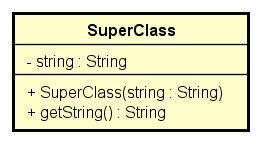
\includegraphics[width=\linewidth]{cd_superclass}
  \caption{SuperClass}
  \label{abb:cd_superclass}

\end{minipage}%
\hspace{.04\linewidth}% Abstand zwischen Bilder
\begin{minipage}[b]{.63\linewidth}


  \centering
  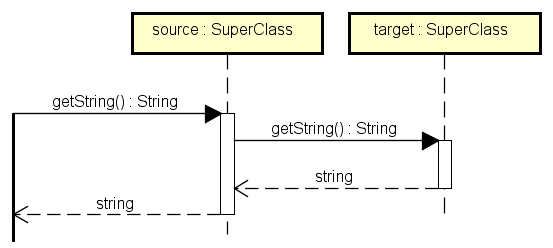
\includegraphics[width=\linewidth]{sd_exact_super}
  \caption{Szenario ExactTypeMatcher}
  \label{abb:sd_exact_super}

\end{minipage}
\end{figure}

\myparagraph{Definition}
\begin{matcherEquivDef}{ExactTypeMatcher}
\matchTyp{A}{exact}{B} \text{ wenn } A = B
\end{matcherEquivDef}
\begin{matcherConvDef}{ExactTypeMatcher}{
Sei $ m $ eine Methode des Typen $ A $ und $ B $.}
\delegate{A.m}{B.m}
\end{matcherConvDef}\\
Ein Beispiel f�r die Verwendung des Matchers ist in \appref{exactMatcherExample} zu finden.
\subsubsection{GenTypeMatcher}\label{genTypeMatcher}
\myparagraph{Szenario}
Dieser Matcher stellt das Matching zwischen zwei Typen her, die in einer Vererbungsbeziehung stehen. Speziell erlaubt dieser Matcher das Matching eines Supertyps als Source-Typen mit einem Subtypen als Target-Typen. In dem Szenario wird neben dem Typ SuperClass aus \abbref{cd_superclass} von einem weiteren Typen SubClass ausgegangen. Dabei stehen diese beiden Typen in einer Vererbungsbeziehnung, die in \abbref{cd_subclass_extends_superclass} dargestellt wird. Der Aufruf einer Methode auf dem Source-Objekt f�hrt zu einer Delgation der Methode an das Target-Objekt (siehe \abbref{sd_gen_super2sub}).
\begin{figure}[H]
\begin{minipage}[b]{.33\linewidth}
  \centering
  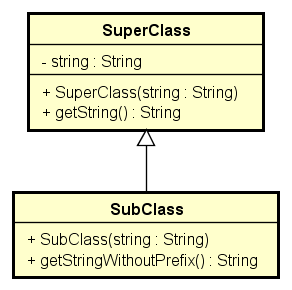
\includegraphics[width=\linewidth]{cd_subclass_extends_superclass}
  \caption{Beziehung zwischen SuperClass und SubClass}
  \label{abb:cd_subclass_extends_superclass}

\end{minipage}%
\hspace{.04\linewidth}% Abstand zwischen Bilder
\begin{minipage}[b]{.63\linewidth}


  \centering
  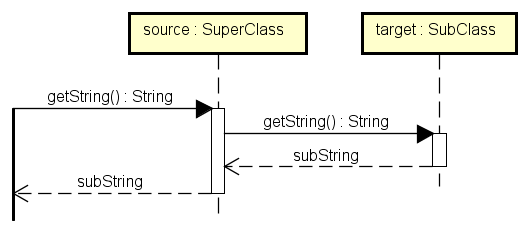
\includegraphics[width=\linewidth]{sd_gen_super2sub}
  \caption{Szenario GenTypeMatcher}
  \label{abb:sd_gen_super2sub}

\end{minipage}
\end{figure}




\myparagraph{Definition}
\begin{matcherEquivDef}{GenTypeMatcher}
\matchTyp{A}{gen}{B} \text{ wenn } \inhTyp{B}{A}
\end{matcherEquivDef}
\begin{matcherConvDef}{GenTypeMatcher}{
Sei $ m $ eine Methode des Typs $ A $, die aufgrund der Vererbung auch von Typ $ B $ bereitgestellt wird.}
\delegate{A.m}{B.m}
\end{matcherConvDef}\\
Ein Beispiel f�r die Verwendung des Matchers ist in \appref{genMatcherExample} zu finden.

\subsubsection{SpecTypeMatcher}\label{specTypeMatcher}
\myparagraph{Szenario}
Analog zum GenTypeMatcher stellt der SpecTypeMatcher ebenfalls das Matching zwischen Typen fest, die in einer Vererbungsbeziehung stehen. Allerdings ist der Source-Typ in diesem Matcher der Subtyp und der Target-Typ der Supertyp. In dem Szenario wird wiederum von den Klassen SuperClass und SubClass aus \abbref{cd_subclass_extends_superclass} ausgegangen. Der Methodenaufruf erfolgt hier aber auf dem Subtypen und wird an den Supertypen delegiert (siehe \abbref{sd_spec_sub2super}).
\myScalableFigure[0.7\linewidth]{sd_spec_sub2super}{Szenario SpecTypeMatcher}{sd_spec_sub2super}
\noindent
Dabei sind zwei Methodenaufrufe auf dem Subtyp beschrieben. W�hrend der Aufruf der Methode getString erfolgreich delegiert werden kann, f�hrt der Aufruf der Methode getStringWithoutPrefix zu einem Laufzeitfehler, da der Matcher keine passende Methode in dem Target-Typ ermitteln kann. Dieses Problem tritt bei allen Methoden auf, die nicht vom Supertyp an den Subtyp vererbt oder �berschrieben wurden.\footnote{Anders gesagt, erm�glicht dieser Matcher einen Downcast, bei dem ein Objekt eines allgemeinen Typen auf einen spezielleren Typen gecastet wird. Das Problem bzgl. des fehlschlagenden Methodenaufrufs in der beschriebene Form ist bei einem Downcast allgegenw�rtig.} Aus diesem Grund muss diese Bedingung in der Definition der Konvertierung dieses Matchers mit aufgenommen werden.
\myparagraph{Definition}
\begin{matcherEquivDef}{SpecTypeMatcher}
\matchTyp{A}{genspec}{B} \text{ wenn } \inhTyp{A}{B}
\end{matcherEquivDef}
\begin{matcherConvDef}{SpecTypeMatcher}{
Sei $ m $ eine Methode des Typs $ A $, die von $ B $ an $ A $ vererbt wurde.}
\delegate{A.m}{B.m}
\end{matcherConvDef}\\
Ein Beispiel f�r die Verwendung des Matchers ist in \appref{specMatcherExample} zu finden.
\subsubsection{WrappedTypeMatcher}\label{wrappedTypeMatcher}
\myparagraph{Szenario}
Die bisherigen Type-Matcher sind in der Lage das Matching f�r zwei Typen festzustellen, ohne daf�r R�cksicht auf deren innere Struktur nehmen zu m�ssen. Dies ist f�r identische oder hierarchisch organisierte Typen auch nicht notwendig. Es ist jedoch auch denkbar, dass sich beiden Typen auf anderem Wegen assoziieren lassen. Ein Beispiel daf�r w�re Boxed- bzw. - noch allgemeiner gefasst - Wrapper-Typen. In \abbref{cd_subclass_subwrapper} sind zwei Klassen dargestellt, die in einer solchen Beziehung zueinander stehen. Bez�glich des Matchings sind auch hier wiederum zwei F�lle zu unterscheiden. Der erste Fall, in dem das Matching des Source-Typen SubClass mit dem Typen eines Attributs wrapped des Traget-Typen SubWrapper festgestellt werden kann, ist in \abbref{sd_wrapped_sub2subwrapped} dargestellt.
\begin{figure}[H]
\begin{minipage}[b]{.33\linewidth}
  \centering
  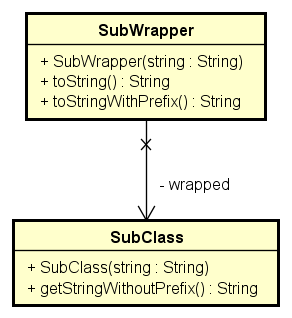
\includegraphics[width=\linewidth]{cd_subclass_subwrapper}
  \caption{Beziehung zwischen SubClass und SubWrapper}
  \label{abb:cd_subclass_subwrapper}

\end{minipage}%
\hspace{.04\linewidth}% Abstand zwischen Bilder
\begin{minipage}[b]{.63\linewidth}


  \centering
  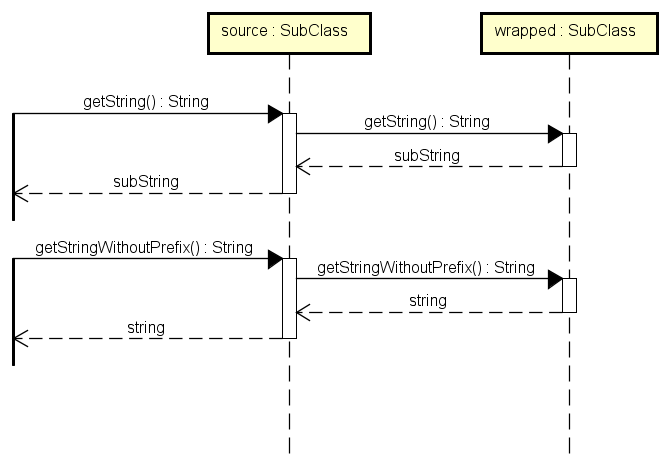
\includegraphics[width=\linewidth]{sd_wrapped_sub2subwrapped}
  \caption{Szenario WrappedTypeMatcher}
  \label{abb:sd_wrapped_sub2subwrapped}

\end{minipage}
\end{figure}
\noindent
Der WrappedTypeMatcher stellt das Matching f�r ein solches Szenario fest. Das Matching der beiden Typen beruht letztendlich auf einem Matching zwischen dem Source-Type und dem Typen eines Attributs des Target-Typs. Der Matcher, �ber den dieses Matching innerhalb des WrappedTypeMatchers festgestellt wird, wird als interner Matcher bezeichnet. In dem Szenario aus \abbref{sd_wrapped_sub2subwrapped} wird als interner Matcher der bereits beschriebene ExactTypeMatcher verwendet, weil der Source-Type und der Typ des Attributs wrapped identisch sind.
\myparagraph{Definition}
\begin{matcherEquivDef}{WrappedTypeMatcher}
\matchTyp{A}{wrapped}{B} \text{ wenn } \exists \selTyp{B}{attr} : \matchTyp{A}{M}{attr}
\end{matcherEquivDef}\\
Der zuvor genannte interne Matcher wird in der Definition mit $M$ beschrieben, was stellvertretend f�r eine Menge von Matchern steht. Als interne Matcher kommen hierbei der ExactTypeMatcher, der GenTypeMatcher und der SpecTypeMatcher in Frage.\\
\begin{matcherConvDef}{WrappedTypeMatcher}{
Sei $m$ eine Methode des Typs $A$. Sei weiterhin $B$ ein Typ, der ein Attribut vom Typ $attr$ enth�lt, f�r den gilt $\matchTyp{A}{M}{attr}$.
}
\delegate{A.m}{(\applyMatcher{A}{attr}).m}
\end{matcherConvDef}\\
Ein Beispiel f�r die Verwendung des Matchers in Bezug auf das o.g. Szenario ist in \appref{wrappedMatcherExample} zu finden. Au�erdem sind dort auch weitere Szenarien aufgef�ht, in denen der GenTypeMatcher oder der SpecTypeMatcher als interner Matcher zur Anwendung kommen.


\subsubsection{WrapperTypeMatcher}\label{wrapperTypeMatcher}
\myparagraph{Szenario}
Dieser Matcher stellt das Pendant zum WrappedTypeMatcher dar. Der Unterschied bzgl. des Szenarios besteht darin, dass nun der Source-Typ derjenige ist, der ein Attribut enth�lt, f�r dessen Typ ein Matching zum Target-Typen �ber den ExactTypeMatcher, den GenTypeMatcher oder den SpecTypeMatcher festgestellt werden kann. F�r das Szenario ist wiederum von den Typen aus \abbref{cd_subclass_subwrapper} auszugehen. Die Delegation der m�glichen Methodenaufrufe am Source-Typen, sind in \abbref{sd_wrapper_subwrapped2sub} abgebildet. Hierbei ist hervorzuheben, dass zur Laufzeit das Objekt vom Target-Typen in das Attribut des Objektes vom Source-Typen injiziert wird. Dies soll in \abbref{sd_wrapper_subwrapped2sub} durch die Bezeichnung des Targets mit wrapped (dem Namen des Attributs) und target dargestellt werden. Eine Methoden-Delegation findet nur dann statt, wenn sie auch im Wrapper-Typen (Source-Typen) implementiert wurde\footnote{Implementierung von SubWrapper: siehe \appref{matcherExamples} \lstref{LST_subwrapper_impl}}.
\myScalableFigure[0.8\linewidth]{sd_wrapper_subwrapped2sub}{Szenario WrapperTypeMatcher}{sd_wrapper_subwrapped2sub}
\myparagraph{Definition}
\begin{matcherEquivDef}{WrapperTypeMatcher}
\matchTyp{A}{wrapper}{B} \text{ wenn } \exists\selTyp{A}{attr} : \matchTyp{B}{M}{attr} 
\end{matcherEquivDef}\\
Wie an dieser Beschreibung zu erkennen ist, werden auch hier wieder ein interner Matcher $M$ verwendet. Analog zum WrappedTypeMatcher kommen auch hier der ExactTypeMatcher, der GenTypeMatcher und der SpecTypeMatcher in Frage.\\
\begin{matcherConvDef}{WrappedTypeMatcher}{
Sei $m$ eine Methode des Typs $A$.
}
\delegate{A.m}{A.m}
\end{matcherConvDef}\\
Ein Beispiel f�r die Verwendung des Matchers in Bezug auf das o.g. Szenario ist in \appref{wrapperMatcherExample} zu finden. Au�erdem sind dort auch weitere Szenarien aufgef�ht, in denen der GenTypeMatcher oder der SpecTypeMatcher als interner Matcher zur Anwendung kommen.

\subsubsection{StructuralTypeMatcher}\label{structTypeMatcher}
Die bisher beschriebene Type-Matcher erlauben lediglich ein Matching zwischen Typen, die syntaktisch miteinander in einer direkten Beziehung stehen. Ein Ziel dieser Arbeit ist es jedoch Typen, die voneinander syntaktisch unabh�ngig sind, miteinander zu matchen, um darauf aufbauend, deren Semantik zu �berpr�fen. Hierf�r soll wie auch in \cite{hummel08} die strukturelle �bereinstimmung der beiden Typen ermittelt und verwendet werden. Diesem Zweck dient der StructuralTypeMatcher.
\myparagraph{Szenario}
Um die grundlegenden Eigenschaften des StructuralTypeMatchers darzustellen, wird von einem Szenario ausgegangen, in dem der Target-Typ (angebotenes Interface) zu jeder Methode des Sources-Typs (ben�tigtes Interface) eine passende Methode anbietet. Eine Kombination von angebotenen Interfaces ist somit in diesem Szenario nicht notwendig.\\\\
\abbref{cd_superrsubp_subrsuperp} zeigt die Typen, von denen in dem folgenden Szenario ausgegangen wird. Hierbei sind zwei Klassen aufgef�hrt, die jeweils zwei Methoden anbieten. Die Parameter- und R�ckgabetypen der Methoden sind aus den Szenarien zu den anderen Matchern bekannt. Die Klasse SuperReturnSubParamClass wird in dem folgenden Szenario als Source-Typ und die Klasse SubReturnSuperWrapperParamClass wird als Target-Typ verwendet. Um die strukturelle �bereinstimmung der beiden Typen festzustellen, muss der StructuralTypeMatcher ein Matching zwischen den Parameter- und R�ckgabetypen der einzelnen Methoden herstellen. Dies erfolgt wiederum �ber interne Type-Matcher. An dieser Stelle k�nnen alle zuvor genannten Type-Matcher als interner Type-Matcher verwendet werden. Die Delegation der Methode-Aufrufe erfolgt dann an die Methode des Target-Objekts, die als �bereinstimmende bzw. passende Methode ermittelt wurde (siehe \abbref{sd_struct}). Da beide Methoden eine unterschiedliche Anzahl von Parametern haben, ist in diesem Beispiel leicht nachzuvollziehen, welche Methoden zusammenpassen. Als interner Type-Matcher wurde in diesem Szenario der GenTypeMatcher verwendet. 
\myBigFigure{cd_superrsubp_subrsuperp}{SuperReturnSubParamClass und SubReturnSuperParamClass}{cd_superrsubp_subrsuperp}
\myBigFigure{sd_struct}{Szenario StructTypeMatcher}{sd_struct}
\myparagraph{Definition}
\begin{matcherEquivDef}{StructuralTypeMatcher}
&\matchTyp{A}{struct}{B} \text{ wenn}\\
&\exists(A.m(MP) : MR) : \exists (B.n(NP):NR):\matchTyp{MP}{P}{NP} \wedge \matchTyp{NR}{R}{MR}
\end{matcherEquivDef}\\
Da die Notation es nicht hergibt, ist zus�tzlich zu erw�hnen, dass die Reihenfolge der Parameter in $m$ und $n$ irrelevant ist.\\
%fuer Formatierung
\\
\begin{matcherConvDef}{StructuralTypeMatcher}{
Sei $m$ eine Methode des Typs $A$.\\
Der R�ckgabetyp von $m$ sei $MR$ und $MP$ der Parametertyp von $m$.\\
Weiterhin sei $n$ eine Methode des Typs $B$.\\
Der R�ckgabetyp von $n$ sei $NR$ und $NP$ der Parametertyp von $n$.
}
\delegate{A.m(MP):MR}{B.n(\applyMatcher{NP}{MP}) : \applyMatcher{MR}{NR}}
\end{matcherConvDef}\\
Ein Beispiel f�r die Verwendung des Matchers in Bezug auf das o.g. Szenario ist in \appref{structMatcherExample} zu finden. Au�erdem sind dort auch weitere Szenarien aufgef�ht, in denen andere Matcher als interner Matcher zur Anwendung kommen.

\subsubsection{Typ- und Methoden-Konvertierungsvarianten}\label{type_meth_conv}
Die Konvertierung der einzelnen Type-Matcher liefert eine Menge von so genannten Typ-Konvertierungsvarianten. Eine Typ-Konvertierungsvariante beschreibt eine M�glichkeit, wie ein Typ in einen anderen konvertiert werden kann. Zu diesem Zweck enth�lt eine Typ-Konvertierungsvariante zwei Arten von Information: 
\begin{enumerate}
\item Objekterzeugungsrelevante Informationen
\item Methodendelegationsrelevante Informationen
\end{enumerate}
Typ-Konvertierungsvarianten werden von einem konkreten Typ-Matcher f�r jede m�gliche Form der �bereinstimmung erzeugt. Ein Matcher erzeugt, wenn �berhaupt, immer nur eine Typ-Konvertierungsvariante.\\\\
Die objekterzeugungsrelevanten Informationen sorgen daf�r, dass das Proxy-Objekt f�r den Source-Typ korrekt erzeugt werden kann.\\\\
Die methodendelegationsrelevanten Informationen werden verwendet um so genannten Methoden-Konvertierungsvarianten zu erzeugen. Diese sorgen daf�r, dass das R�ckgabe-Objekt und die Parameter-Objekte beim Methodenaufruf korrekt konvertiert werden und dass der Aufruf an die richtige Methode des Target-Typs delegiert wird.\\\\
Speziell der StructuralTypeMatcher erm�glicht es, zu einer Methode des Source-Typen mehrere methodendelegationsrelevanten Informationen zu erhalten. Das liegt daran, dass dieser Matcher alle Methoden des Source- und des Target-Typen miteinander auf �berstimmung �berpr�ft. Dabei kann es vorkommen, dass eine Methode des Source-Typen mit mehreren Methoden des Target-Typen - oder umgekehrt - �bereinstimmt.
In \abbref{konvar_voll} ist dieser Zusammenhang f�r ein angebotenes Interface AIv und einem erwarteten Interface EI, welche jeweils zwei Methoden enthalten (AM * bzw. EM *), skizziert. Hier wird angenommen, dass jede der angebotenen Methoden strukturell mit jeder der erwarteten Methoden �bereinstimmen w�rde. Dementsprechend enth�lt die Typ-Konvertierungsvariante (TKV) methodendelegationsrelevante Informationen, aus denen insgesamt 4 Methoden-Konvertierungsvarianten erzeugt werden, wovon jede eine Konvertierung entlang der eingezeichneten Pfeile erm�glicht.\\\\
Dabei gilt jedoch, aufgrund der �berlegungen zur Kombination von angebotenen Komponenten (siehe auch \abbref{combinated_components}), dass eine Typ-Konvertierungsvariante nicht zu jeder der erwarteten Methoden solche methodendelegationsrelevanten Informationen enth�lt. \abbref{konvar_unv} zeigt einen solchen Fall mit dem angebotenen Interface AIu.
\begin{figure}[H]
\begin{minipage}[b]{.48\linewidth}
  \centering
  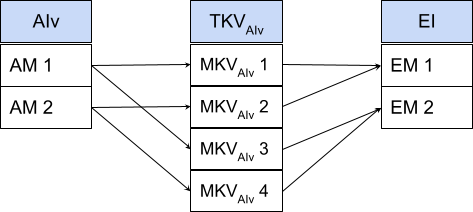
\includegraphics[width=\linewidth]{konvar_voll}
  \caption{Typ- und Methoden-Konvertierungsvarianten von AIv}
  \label{abb:konvar_voll}

\end{minipage}%
\hspace{.04\linewidth}% Abstand zwischen Bilder
\begin{minipage}[b]{.48\linewidth}


  \centering
  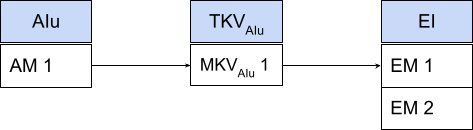
\includegraphics[width=\linewidth]{konvar_unv}
  \caption{Typ- und Methoden-Konvertierungsvarianten von AIu}
  \label{abb:konvar_unv}

\end{minipage}
\end{figure}


\section{2. Stufe - Semantische Evaluation}\label{sem_eval}
Sofern alle Typ-Konvertierungsvarianten des erwarteten Interfaces bzgl. einer Menge von angebotenen Interfaces in der 1. Stufe ermittelt wurden, k�nnen die ben�tigten Komponenten erzeugt und getestet werden.\\\\
Diese Pr�fung wird �ber die vorab spezifizierten Testf�lle des erwarteten Interfaces vorgenommen. In einem vorherigen Abschnitt wurde schon kurz beschrieben, wie eine solche Testklasse aufgebaut ist. In diesem Abschnitt wird beschrieben, wie die zu testenden ben�tigten Komponenten ermittelt werden und wie die Tests durchgef�hrt werden. 
Dies erfolgt in 6 Schritten, die im Folgenden erl�utert werden. Eine schmatische Darstellung der Semantischen Evaluation ist \abbref{flowchart_sem_eval} zu entnehmen.
\myBigFigure{flowchart_sem_eval}{Schema der semantischen Evaluation}{flowchart_sem_eval}

\subsubsection{Ermittlung der Testklassen zum erwarteten Interface}\label{sem_eval_step1}
Die Ermittlung der Testklassen erfolgt �ber die Annotation @QueryTypeTestReference, welche im erwarteten Interface spezifiziert wird. Von diesen Testklassen wird ein Testobjekt �ber den Default-Konstruktor erzeugt.
\subsubsection{Schritt 2: Kombination von Typ-Konvertierungsvarianten}\label{sem_eval_step2}
In diesem Schritt werden die ermittelten Typ-Konvertierungsvarianten miteinander kombiniert, was einer Kombination der angebotenen Interfaces gleicht. Die Anzahl $k$ der zu kombinierenden Typ-Konvertierungsvarianten kann jedoch variieren. Wenn $|EM|$ die Anzahl der Methoden im erwarteten Interface ist, gilt f�r $k$:
\begin{align*}
1 \leq k \leq |EM|
\end{align*}
\noindent
Da $k$ variabel ist, wird dieser Schritt zusammen mit allen folgenden Schritten mitunter mehrfach durchlaufen. Die Nummer des jeweiligen Iterationsschrittes wird mit $k$ gleichgesetzt. Somit wird die Anzahl der zu kombinierenden Typ-Konvertierungsvarianten mit jedem Durchlauf erh�ht. \abbref{tkv_alv_alu_1} zeigt die Kombinationen von Typ-Konvertierungsvarianten, die sich - bezogen auf die Beispiele aus \abbref{konvar_voll} und \abbref{konvar_unv} - im ersten Durchlauf ergeben. Im zweiten Durchlauf w�rde sich nur eine Kombination von Typ-Konvertierungsvarianten ergeben, da die beiden Typ-Konvertierungsvarianten von AIv und AIu miteinander kombiniert werden (siehe \abbref{comb_tkv_alv_alu_1}).



\begin{figure}[H]
\begin{minipage}[b]{.48\linewidth}
  \centering
  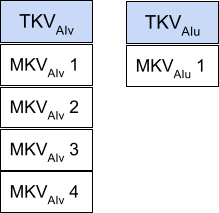
\includegraphics[width=.6\linewidth]{tkv_alv_alu_1}
  \caption{Kombinationen von Typ-Konvertierungsvarianten von AIu und AIv im ersten Durchlauf}
  \label{abb:tkv_alv_alu_1}

\end{minipage}%
\hspace{.04\linewidth}% Abstand zwischen Bilder
\begin{minipage}[b]{.48\linewidth}


  \centering
  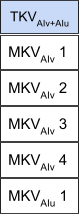
\includegraphics[width=.2\linewidth]{comb_tkv_alv_alu_1}
  \caption{Kombinationen von Typ-Konvertierungsvarianten von AIu und AIv im zweiten Durchlauf}
  \label{abb:comb_tkv_alv_alu_1}

\end{minipage}
\end{figure}

\noindent
So berechnet sich die Anzahl an ermittelten Kombinationen von Typ-Konvertierungsvarianten  ($|KombTKV|$) f�r jeden Durchlauf $k$ in Abh�ngigkeit von der Anzahl der in der 1. Stufe ermittelten Typ-Konvertierungsvarianten ($|TKV|$) wie folgt:
\begin{align*}
|KombTKV| = \frac{|TKV|! }{ (|TKV| - k)! * k!}
\end{align*}


\subsubsection{Schritt 3: Erzeugen einer ben�tigten Komponente}\label{sem_eval_step3}
Eine ben�tigte Komponente besteht aus einer Kombination von Methoden-Konvertierungsvarianten, wobei f�r jede erwartete Methode genau eine Methoden-Konvertierungsvariante innerhalb der ben�tigten Komponente existiert.\\\\
F�r die Ermittlung der Kombinationen von Methoden-Konvertierungsvarianten wird eine Kombination von Typ-Konvertierungsvarianten aus der Ergebnismenge des zweiten Schrittes im aktuellen Durchlauf  selektiert. Die daraus erzeugten Methoden-Konvertierungsvarianten werden hinsichtlich der Methoden aus dem erwarteten Interface miteinander kombiniert.\\\\
F�r die erste Kombination von Typ-Konvertierungsvarianten, die \abbref{tkv_alv_alu_1} zu entnehmen ist ($TKV_{AIv}$),  k�nnen folgende Kombinationen von Methoden-Konvertierungsvarianten erzeugt werden (siehe \abbref{comb_mkv_alv_1}).
\myBigFigure{comb_mkv_alv_1}{Kombinationen von Methoden-Konvertierungsvarianten AIv}{comb_mkv_alv_1}
\noindent
Analog dazu wird f�r die zweite Kombination von Typ-Konvertierungsvarianten, die \abbref{tkv_alv_alu_1} zu entnehmen ist ($TKV_{AIu}$), folgende Kombination von Methoden-Konvertierungsvarianten erzeugt (siehe \abbref{comb_mkv_alu_1}).\\\\
Ausgehend von der Kombination von Typ-Konvertierungsvarianten aus \abbref{comb_tkv_alv_alu_1} ($TKV_{AIu+AIv}$), sind in \abbref{comb_mkv_alu_alv} die daraus resultieren Methoden-Konvertierungsvarianten dargestellt.Zu beachten ist, dass die ersten vier Kombinationen bereits im vorherigen Durchlauf erzeugt wurden (siehe \abbref{comb_mkv_alv_1}) und dementsprechend auch getestet wurden.



\begin{figure}[H]
\begin{minipage}[b]{.38\linewidth}
  \centering
  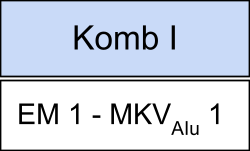
\includegraphics[width=.6\linewidth]{comb_mkv_alu_1}
  \captionof{figure}{Kombinationen von Methoden-Konvertierungsvarianten AIu}
  \label{abb:comb_mkv_alu_1}

\end{minipage}%
\hspace{.04\linewidth}% Abstand zwischen Bilder
\begin{minipage}[b]{.58\linewidth}


  \centering
  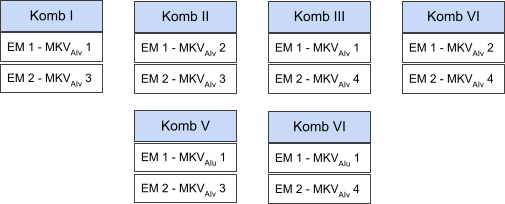
\includegraphics[width=\linewidth]{comb_mkv_alu_alv}
  \captionof{figure}{Kombinationen von Methoden-Konvertierungsvarianten AIu+AIv}
  \label{abb:comb_mkv_alu_alv}

\end{minipage}
\end{figure}


\noindent


\noindent
Im Allgemeinen l�sst sich sagen, dass die Anzahl der Kombinationen von Methoden-Konvertierungsvarianten von der Anzahl der Methoden im erwarteten Interface ($|EM|$) und der Anzahl von Methoden-Konvertierungsvarianten ($|MKV|$), die aus der selektierten Kombination von Typ-Konvertierungsvarianten erzeugt werden k�nnen. Da aus einer Kombination von Methoden-Konvertierungsvarianten jeweils eine ben�tigte Komponente erzeugt werden kann, gilt f�r die Anzahl der ben�tigten Komponenten ($|Komb_{ben}|$) dasselbe. Im schlimmsten Fall berechnet sich die Anzahl der ben�tigten Komponenten wie folgt:
\begin{align*}
|Komb_{ben}| = |Komb_{MKV}| = \frac{|MKV|!}{(|MVK| - |EM|)!*|EM|!}
\end{align*}


\subsubsection{Injizieren der ben�tigten Komponente}\label{sem_eval_step4}
Der Setter f�r die Setter-Injection wird in der Testklasse �ber die Annotation @QueryTypeInstanceSetter ermittelt. Danach wird diese Methode auf dem Testobjekt mit der ben�tigten Komponente als Parameter aufgerufen. 
\subsection{Schritt 5: Durchf�hren der Tests}\label{sem_eval_step5}
Die Testf�lle aus der Testklasse werden �ber die Annotation @QueryTypeTest ermittelt und sequentiell ausgef�hrt. Als Ergebnis der Testausf�hrung f�r eine ben�tigte Komponente wird ein Objekt des Typs TestResult zur�ckgegeben. Tritt bei der Testausf�hrung eine Exception auf, wird diese im TestResult-Objekt hinterlegt. Im Anschluss wird das TestResult-Objekt direkt zur�ckgegeben, um die Ausf�hrung der �brigen Tests zu verhindern. Wenn ein Test mit positivem Ergebnis durchgef�hrt wird, wird das Attribut passedTests im TestResult-Objekt inkrementiert. Sollten alle Tests erfolgreich durchgef�hrt worden sein, wird das TestResult-Objekt zur�ckgegeben.
\myparagraph{Umgang mit kombinierten angebotenen Komponenten}
Ab dem zweiten Durchlauf werden werden die ben�tigten Komponenten in Schritt 3 aus Kombinationen von Typ-Konvertierungsvarianten mehrere angebotener Interfaces erzeugt. Das f�hrt dazu, dass die Methodenaufrufe auf dem erwarteten Interface an unterschiedliche angebotene Komponenten delegiert werden. Hierbei kann der Fall eintreten, dass mehrere dieser Methoden von der Semantik her auf den gleichen Daten operieren m�ssen, die Aufrufe dieser jedoch an unterschiedliche Komponenten delegiert werden, welche auch auf unterschiedlichen Daten operieren.\\\\
Ein Beispiel hierf�r w�re ein Stack, der durch das erwartete Interface Stack beschrieben. Dieses enth�lt eine push und eine pop Methoden mit der ein Element im Stack hinzugef�gt bzw. entfernt werden kann (siehe \abbref{expected_stack}). Hierbei ist anzunehmen, dass die beiden Methoden auf denselben Daten arbeiten, sodass nach dem Hinzuf�gen eines Elements a (push(a)) und dem darauf folgenden Aufruf der Methode pop() als R�ckgabewert wieder das zuvor hinzugef�gte Element a geliefert wird (siehe \abbref{sd_stack_1}). Wenn die beiden Methoden-Aufrufe jedoch an zwei unterschiedliche Objekte StackA und StackB delegiert werden, die auf unterschiedlichen Daten operieren, dann w�rde dieses Verhalten nicht nachgewiesen werden k�nnen (siehe \abbref{sd_stack_2}).

\begin{figure}[H]
\begin{minipage}[b]{.24\linewidth}
  \centering
  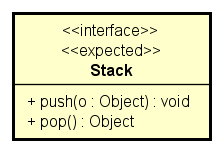
\includegraphics[width=\linewidth]{expected_stack}
  \captionof{figure}{Erwartetes Interface Stack}
  \label{abb:expected_stack}

\end{minipage}%
\hspace{.04\linewidth}% Abstand zwischen Bilder
\begin{minipage}[b]{.72\linewidth}


  \centering
  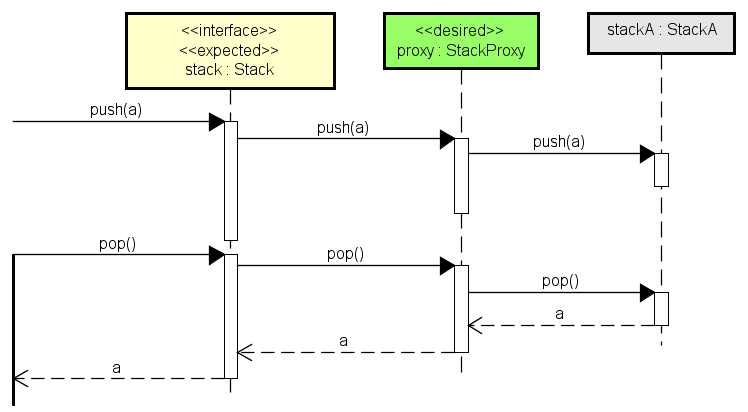
\includegraphics[width=\linewidth]{sd_stack_1}
  \captionof{figure}{Delegation der Stack-Methoden an genau eine angebotene Komponente}
  \label{abb:sd_stack_1}

\end{minipage}
\end{figure}


%\myBigFigure{expected_stack}{Erwartetes Interface Stack}{expected_stack}
%\myBigFigure{sd_stack_1}{Delegation der Stack-Methoden an genau eine angebotene Komponente}{sd_stack_1}
\myBigFigure{sd_stack_2}{Delegation der Stack-Methoden an unterschiedliche angebotene Komponenten}{sd_stack_2}
\noindent
In einem solchen Fall sollte der Zusammenhang dieser erwarteten Methoden in den Tests spezifiziert werden, sodass diese besonderen semantischen Anforderungen in diesem Schritt evaluiert werden k�nnen. \lstref{LST_StackTest} zeigt ein Beispiel bezogen auf das Szenario aus \abbref{sd_stack_1}.
\begin{lstlisting}[{caption = Testklasse f�r ein erwartetes Interfaces Stack
},{label = LST_StackTest}]
public class StackTest {

  private Stack stack;

  @QueryTypeInstanceSetter
  public void setProvider( Stack stack ) {
    this.stack = stack;
  }

  @QueryTypeTest
  public void pushPop() {
    Object a = new Object();
    stack.push( a );
    Object evalObj = stack.pop();
    assertTrue( a == evalObj );
  }

}
\end{lstlisting}

\subsubsection{Schritt 6: Auswertung des Testergebnisses}\label{sem_eval_step6}
Sofern alle Tests erfolgreich durchgelaufen sind, wird die aktuell selektierte ben�tigte Komponente als passend bewertet und als Ergebnis des Explorationsalgorithmus zur�ckgegeben.\\\\
Sollte einer der Tests nicht erfolgreich sein, wird die semantische Evaluation ab Schritt 3 (siehe \ref{sem_eval_step3}) wiederholt. Sofern keine ben�tigten Komponenten mehr erzeugt werden k�nnen, ist die Suche nach einer passenden Komponente gescheitert.\\\\
Da die Suche zur Laufzeit ausgef�hrt wird, reicht es, wenn eine passende Komponente gefunden wird. Selbst wenn es mehrere passende Komponenten geben sollte, g�be es in dem beschriebenen Verfahren keine M�glichkeit festzustellen, welche die semantischen Anforderungen besser erf�llt. Zwar w�ren k�nnte man die passenden Komponenten hinsichtlich der ben�tigten Systemressourcen untersuchen. Aufgrund der Vielzahl von m�glichen Kombinationen (siehe \ref{sem_eval_step2} und \ref{sem_eval_step3}) rechtfertigt der daf�r notwendige Aufwand den daraus resultierenden Performancegewinn vermutlich nicht.


\section{Heuristiken}\label{sec_heuristics}
Als \Gls{Heuristik}en werden in dieser Arbeit Verfahren bezeichnet, durch die die Lösung eines Problems beschleunigt werden kann, indem neu gewonnene Erkenntnisse beim Finden der Lösung berücksichtigt werden. Konkret bedeutet dies, dass die oben beschriebene \emph{semantische Evaluation} durch diese Verfahren beschleunigt werden soll.
\\\\
Die \Gls{Heuristik}en, die in den Abschnitten \ref{sec_lmf} und \ref{sec_pttf} beschrieben werden, haben zum Ziel, die Reihenfolge, in der die \emph{Proxies} hinsichtlich der vordefinierten Tests geprüft werden, so anzupassen, dass ein valider \emph{Proxy} möglichst früh geprüft wird. Die dritte \Gls{Heuristik}, die im Abschnitt \ref{sec_bl_nmc} beschrieben wird, beschreibt ein Ausschlussverfahren.
\\\\
Für die Verwendung der \Gls{Heuristik}en wird der Algorithmus aus Listing \ref{lst_semEval} erweitert. Diese Erweiterung beinhaltet die Verwaltung der neu gewonnenen Erkenntnisse sowie die Anwendung der \Gls{Heuristik}en auf die zu generierenden bzw. generierten \emph{Proxies}. 
\\\\
In den folgenden Abschnitten werden die \Gls{Heuristik}en und die dafür notwendigen Anpassungen an den jeweiligen Funktionen beschrieben. Der Pseudo-Code für die \emph{semantische Evaluation} inklusive der Verwendung aller vorgestellten \Gls{Heuristik}en ist im Anhang \ref{app_semEvalMitAllenHeuristiken} zu finden.


\subsection{Beachtung des Matcherratings (LMF)}\label{sec_lmf}
Bei dieser \Gls{Heuristik}, welche den Namen \emph{low matcherrating first} (kurz: \emph{LMF}) trägt, werden die Mengen von \emph{Target-Typen}, aus denen die \emph{Proxies} erzeugt werden, auf der Basis eines so genannten \emph{Matcherratings} bewertet. Bei dem \emph{Matcherrating} einer solchen Menge handelt es sich um einen numerischen Wert, auf dessen Basis entschieden werden kann, für welche Menge von \emph{Target-Typ} die Generierung und Prüfung der \emph{Proxies} zuerst vollzogen werden soll.
\\\\
Um das \emph{Matcherrating} zu ermitteln, wird für jede Matchingrelation bzw. für jeden Matcher aus Abschnitt \ref{sec_matcher} ein \emph{Basisrating} vergeben. Folgende Funktion beschreibt das \emph{Basisrating} für das Matching zweier Typen $S$ und $T$:
\begin{gather*}
\mathit{base(S,T)} :=  \left\{ 
				\begin{array}{l}
					100 \text{ wenn } S \Rightarrow_{exact}  T  \\
					200 \text{ wenn } S \Rightarrow_{gen}  T  \\
					200 \text{ wenn } S \Rightarrow_{spec}  T  \\
					300 \text{ wenn } S \Rightarrow_{contained}  T   \\
					300 \text{ wenn } S \Rightarrow_{container}  T  				
				\end{array}             
	\right.
\end{gather*}
\noindent
Dabei ist zu erwähnen, dass einige der oben genannten Matcher über dasselbe \emph{Basisrating} verfügen. Das liegt daran, dass sie technisch jeweils gemeinsam umgesetzt wurden.\footnote{Der \emph{GenTypeMatcher} und der \emph{SpecTypeMatcher} wurden gemeinsam in der Klasse $\texttt{GenSpecTypeMatcher}$ umgesetzt. Der \emph{ContentTypeMatcher} und der \emph{ContainerTypeMatcher} wurden gemeinsam in der Klasse $\texttt{ContainerTypeMatcher}$ umgesetzt. (siehe auch Abschnitt \ref{impl_sigma})}
\\\\
Wie an der Funktion $\mathit{base}$ zu erkennen ist, wird das \emph{Matcherrating} für Typen, die über den \emph{StructuralTypeMatcher} gematcht wurden, nicht spezifiziert. Dieses muss berechnet werden. Die Basis dafür bildet ein \emph{Matcherrating}, welches für die gematchten Methoden ermittelt wird. Hierzu sei die Funktion $\mathit{bases_{method}}$ für zwei Methoden $\mathit{mR}$ und $\mathit{mT}$ mit $\mathit{mR} \Rightarrow_{method} \mathit{mT}$ wie folgt definiert:
\begin{gather*}
\mathit{bases_{method}(mR,mT)} := \begin{array}{l|l}
\mathit{base(ret(mR), ret(mT))} \cup \mathit{ }
&
\{\mathit{pR_1,...,pR_n}\} = \mathit{params(mR)} \wedge \mathit{ }
\\
\bigcup\limits_{i=1}^{n} \mathit{base(pR_i,pT_i)}
&
\{\mathit{pT_1,...,pT_n}\} = \mathit{params(mT)}
\end{array} 
\end{gather*}
\noindent
Darauf aufbauend kann die Funktion $\mathit{mRating}$ für die beiden Methoden $\mathit{mR}$ und $\mathit{mT}$ definiert werden. Hierzu seien folgende Hilfsfunktionen definiert:
\begin{gather*}
\mathit{sum(\{v_1,...v_n\})} := \sum_{i=1}^{n}v_i
\\
\mathit{max(\{v_1,...,v_n\})} := 
\begin{array}{l|l}
v_{m}
&
1 \leq m \leq n  \wedge \forall i \in  \{1,...,n\}: v_i \leq v_{m}
\end{array}
\\    
\mathit{min(\{v_1,...,v_n\})} := 
\begin{array}{l|l}
v_{m}
&
1 \leq m \leq n  \wedge \forall i \in  \{1,...,n\}: v_i \geq v_{m} 
\end{array}  
\end{gather*}
\noindent
In dieser Arbeit werden vier Varianten für diese Definition von $\mathit{mRating}$ vorgeschlagen, die in Abschnitt \ref{sec_evalLMF} evaluiert werden sollen.
\paragraph{Variante 1: Durchschnitt ($\mathit{mRating}_1$)}

\begin{gather*}
\mathit{mRating_1(mR,mT)} := \frac{\mathit{sum(base_{method}(mR,mT))}}{|\mathit{params(mR)}|+1}
\end{gather*}

\paragraph{Variante 2: Maximum ($\mathit{mRating}_2$)}

\begin{gather*}
\mathit{mRating_2(mR,mT)} := \mathit{max(bases_{method}(mR,mT))}
\end{gather*}

\paragraph{Variante 3: Minimum ($\mathit{mRating}_3$)}

\begin{gather*}
\mathit{mRating_3(mR,mT)} := \mathit{min(bases_{method}(mR,mT))}
\end{gather*}

\paragraph{Variante 4: Durchschnitt aus Minimum und Maximum ($\mathit{mRating}_4$)}

\begin{gather*}
\mathit{mRating_4(mR,mT)} := \frac{\mathit{max(bases_{method}(mR,mT))}+\mathit{min(bases_{method}(mR,mT))}}{2}
\end{gather*}
\noindent
In einem \emph{provided Typ} $T$ sind mitunter mehrere Methoden deklariert, die ein Matching zu einer Methode $m$ aufweisen. Für die Bestimmung des \emph{Matcherratings} sei hierbei nur das kleinste \emph{Matcherrating} jener Methoden aus $P$ relevant. Das \emph{minimale Matcherrating} einer solchen Methode wird durch folgende Funktion beschrieben\footnote{Da die Varianten der Funktion $\mathit{mRating}$ in $\mathit{minMRating}$ flexibel verwendet werden können, wurde für $\mathit{mRating}$ das Subskript $*$ verwendet.}
\begin{gather*}
\mathit{minMRating(m, T)} := 
	\begin{array}{l|l}
\mathit{min(mRating_*(m'_1),}
&
\{\mathit{m'_1,...,m'_n}\} =
\\
\mathit{...,mRating_*(m'_n))}
&
\mathit{structM_{target}(m, T)}
\end{array}
\end{gather*}
\noindent
Für einen \emph{required Typ} $R$ und einem \emph{provided Typ} $T$ wird die Menge dieser \emph{minimalen Matcherratings} je Methode $m \in \mathit{structM(R)}$ über folgende Funktion definiert:
\begin{gather*}
\mathit{minMRatings(R,T)} := \left\{
\begin{array}{l|l}
	\mathit{minMRating(m,T)}
	& 
	m \in \mathit{structM(R,T)}
\end{array}
\right\}
\end{gather*}
\noindent
In einer Bibliothek $L$ wird die Ermittlung des \emph{Matcherratings} eines \emph{required Typs} $R$ und einer Menge von \emph{provided Typen} $\{T_1,...,T_n\}$ mit $\{T_1,...,T_n\} \in \mathit{cover(R,L)}$ über die Funktion $\mathit{rating}$ beschrieben. Auch hierfür werden in dieser Arbeit insgesamt 4 Varianten vorgeschlagen, die in Kapitel \ref{chap_evaluation} evaluiert werden sollen.
\paragraph{Variante 1: Durchschnitt ($\mathit{rating}_1$)}

\begin{gather*}
\mathit{rating_1(R,\{T_1,...,T_n\})} := \frac{\mathit{sum(minMRatings(R,T_1),...,minMRatings(R,T_n))}}{\sum_{i=1}^{n}|\mathit{structM(R,T_i)}|}
\end{gather*}

\paragraph{Variante 2: Maximum ($\mathit{rating}_2$)}

\begin{gather*}
\mathit{rating_2(R,\{T_1,...,T_n\})} := \mathit{max(minMRatings(R,T_1),...,minMRatings(R,T_n))}
\end{gather*}

\paragraph{Variante 3: Minimum ($\mathit{rating}_3$)}

\begin{gather*}
\mathit{rating_3(R,\{T_1,...,T_n\})} := \mathit{min(minMRatings(R,T_1),...,minMRatings(R,T_n))}\end{gather*}

\paragraph{Variante 4: Durchschnitt aus Minimum und Maximum ($\mathit{rating}_4$)}

\begin{gather*}
\mathit{rating_4(R,\{T_1,...,T_n\})} := 
	\frac{\splitfrac{\mathit{min(minMRatings(R,T_1),...,
	minMRatings(R,T_n))}}
	{+ \mathit{max(minMRatings(R,T_1),...,minMRatings(R,T_n))}}}{2}	
\end{gather*}
\noindent
Da die Funktion $\mathit{rating}$ von $\mathit{mRating}$ abhängt und für $\mathit{mRating}$ 4 Varianten vorgeschlagen wurden, ergeben sich insgesamt 16 Varianten für die Definition von $\mathit{rating}$. Diese Varianten (1.1 - 4.4) sind in der Tabelle \ref{tab_matcherratingvarianten} mit den Kombinationen der Varianten für $\mathit{mRating}$ und $\mathit{rating}$ aufgeführt.

\begin{table}[h!]
\centering
\small
\begin{tabular}{|c|c|c|c|c|c|c|c|c|c|c|c|c|c|c|c|c|}
\hline
\hline
\textbf{Variante} & 1.1 & 1.2 & 1.3 & 1.4 
& 2.1 & 2.2 & 2.3 & 2.4 
& 3.1 & 3.2 & 3.3 & 3.4 
& 4.1 & 4.2 & 4.3 & 4.4 
\\
\hline
$\mathit{rating}_{*}$& 1 & 1 & 1 & 1
& 2 & 2 & 2 & 2 
& 3 & 3 & 3 & 3 
& 4 & 4 & 4 & 4 
\\
\hline
$\mathit{mRating}_{*}$ & 1 & 2 & 3 & 4 
& 1 & 2 & 3 & 4 
& 1 & 2 & 3 & 4 
& 1 & 2 & 3 & 4 
\\
\hline
\hline
\end{tabular}
\caption{Varianten für die Ermittlung des Matcherratings einer Menge von \emph{provided Typen}}
 \label{tab_matcherratingvarianten}
\end{table}
\noindent
Zur Anwendung der \Gls{Heuristik} muss das \emph{Matcherrating} bei der Generierung der \emph{Proxies} aus den jeweiligen Mengen von \emph{provided Typen} beachtet werden. Dabei sollte die Liste der Mengen von \emph{provided Typen}, die über die Funktion $\mathit{targetSets}$ abgebildet wird (siehe Abschnitt \ref{sec_semEvalAlgo}) und über die in der Methode $\texttt{semanticEval}$ (siehe Listing \ref{lst_semEval}) iteriert wird, entsprechend dem \emph{Matcherrating} sortiert werden. Dadurch werden in der Methode $\texttt{evalProxies}$ (siehe Listing \ref{lst_semEval}) zuerst die \emph{Proxies} generiert und geprüft, die auf Basis einer Menge von \emph{provided Typen} mit dem kleinsten \emph{Matcherrating} erzeugt wurden.
\\\\
Listing \ref{lst_lmf} zeigt die Anpassungen der Methode $\texttt{relevantProxies}$ auf Basis der Implementierung der \emph{semantischen Evaluation} aus Listing \ref{lst_semEval}. Für die Sortierung der Liste von \emph{Proxies} wurde in der Methode $\texttt{LMF}$ exemplarisch das \Gls{bsort}-Verfahren verwendet.

\begin{lstlisting}[style = pseudo, caption=Semantische Evaluation mit Heuristik \emph{LMF}, captionpos=b, label = lst_lmf]
function semanticEval( R, T, tests ){
 for( anzahl = 1; anzahl <= $\mathit{maxTargets( R )}$; i++ ){
  targetSets = $\mathit{targetSets( T, anzahl )}$
  sortedSets = LMF( R, targetSets )		
  for( targets : sorted ){
   relProxies = $\mathit{proxies( R, targets )}$
   proxy = evalProxies( relProxies, tests )	
   if( proxy != null ){
    return proxy
   }
  }
 }
 return null;
}

function LMF( R, targets ){
 for( n=targets.size(); n>1; n--){
  for( i=0; i<n-1; i++){
   if( $\mathit{rating(R,}$ targets[i] $)$ < $\mathit{rating(R,}$ targets[i+1] $)$ ){
    tmp = targets[i]
    targets[i] = targets[i+1]
    targets[i+1] = tmp
   }
  }
 }	
 return targets
}
\end{lstlisting}


\subsection{Beachtung positiver Tests (PTTF)}\label{sec_pttf}
Das Testergebnis, welches bei Applikation eines Testfalls für einen \emph{Proxy} ermittelt wird, ist maßgeblich von den \emph{Methoden-Delegationen} des \emph{Proxies} abhängig. Jede \emph{Methoden-Delegation} $\mathit{MD}$ enthält einen Typ in dem die \emph{Delegationsmethode} deklariert wurde. Dieser Typ befindet sich im Attribut $\texttt{MD.del.delTyp}$. Im Fall der \emph{sturkturellen Proxies}, handelt es sich bei diesem Typ um einen der \emph{Target-Typen} des \emph{Proxies}. Bezüglich der \emph{Target-Typen} möglicher \emph{struktureller Proxies} gilt folgendes Theorem\footnote{Der Beweis ist in Anhang \ref{app_proofs} zu finden.}
\begin{theorem}\label{lemma_wiederholteTargets}
Sei $R$ ein \emph{required Typ} aus einer Bibliothek $L$. Sei weiterhin $\mathit{C} = \mathit{cover(R,L)}$. Ferner seien $\mathit{TM} \in \mathit{C}$ und $\mathit{TM'} \in \mathit{C}$ mit $\mathit{proxies_{struct}(R,TM)} \neq \emptyset$ sowie $\mathit{proxies_{struct}(R,TM')} \neq \emptyset$ und $|\mathit{TM}| < |\mathit{TM'}|$ gegeben.
\\\\
Dann gilt:
\begin{gather*}
\forall \mathit{T} \in \mathit{TM}: \exists \mathit{TM''} \in \mathit{targetSets(C,|\mathit{TM'}|)}: \mathit{proxies_{struct}(R,TM'')} \neq \emptyset \wedge \mathit{T} \in \mathit{TM''} 
\end{gather*}
\end{theorem}
\noindent
In Bezug auf die \emph{Proxies}, die bei der \emph{semantischen Evaluation} in mehreren Durchläufen geprüft werden sollen, bedeutet das Folgendes: Die einzelnen \emph{Target-Typen} der \emph{Proxies}, die innerhalb eines Durchlaufs geprüft wurden, sind auch in den \emph{Target-Typen} der \emph{Proxies} enthalten, die in einem späteren Durchlauf geprüft werden - sofern solche \emph{Proxies} überhaupt existieren.
\\\\
Für die in diesem Abschnitt beschriebene \Gls{Heuristik} mit dem Namen \emph{positive tested targets first} (kurz: \emph{PTTF}) ist das Ergebnis einzelner Tests in Bezug auf einen \emph{Proxy} $P$ relevant. Wenn ein Testfall mit einem \emph{Proxy} $P$ erfolgreich durchgeführt wurde, dann sollte die Reihenfolge der zu prüfenden \emph{Proxies} späterer Durchläufe so angepasst werden, dass die \emph{Proxies}, die einen \emph{Target-Typen} des \emph{Proxies} $P$ verwenden, im weiteren Verlauf zuerst geprüft werden.
\newpage
\noindent
Dafür sind auf Basis von Listing \ref{lst_semEval} mehrere Anpassungen bzgl. der Implementierung der Methode $\texttt{evalProxies}$ von Nöten:
\begin{enumerate}
\item 
Die \emph{Target-Typen} der \emph{Proxies}, mit denen mind. ein Testfall erfolgreich durchgeführt werden konnte, müssen in einer globalen Variable ($\texttt{prioTargets}$) hinterlegt werden.

\item 
Die Liste der \emph{Proxies}, die der Methode $\texttt{evalProxies}$ als Parameter übergeben wird, muss so sortiert werden, dass die \emph{Proxies}, mit den \emph{Target-Typen}, die in der globalen Variable ($\texttt{prioTargets}$) hinterlegt wurden, zuerst getestet werden. 

\item 
Die Liste der \emph{Proxies}, über die innerhalb der Methode $\texttt{evalProxies}$ iteriert wird, kann bzgl. ihrer Reihenfolge bereits dann optimiert werden, wenn mind. einer der Testfälle für den aktuellen \emph{Proxy} erfolgreich durchgeführt wurde. Dazu müssen jedoch die \emph{Proxies}, die bereits innerhalb der Methode getestet wurden, in einer lokalen Variable ($\texttt{tested}$) hinterlegt werden. Dann kann die Methode rekursiv mit den \emph{Proxies}, die noch nicht getestet wurden, aufgerufen werden. So werden die darin enthaltenen Elemente aufgrund der 2. Anpassung erneut sortiert.
\end{enumerate}  
In Listing \ref{lst_pttf} sind die oben genannten Anpassungen im Vergleich zu Listing \ref{lst_semEval} zu entnehmen.
\newpage
\begin{lstlisting}[style = pseudo, caption = Semantische Evaluation mit Heuristik \emph{PTTF}, captionpos = b, label = lst_pttf]
prioTargets = []

function evalProxies( proxies, tests ){
 tested = []
 sorted = PTTF( proxies )
 for( proxy : sorted ){
  passedTests = 0
  evalProxy( proxy, tests )
  if( passedTests == tests.size ){
   return proxy
  }
  else{
   tested.add( proxy )
   if( passedTests > 0 ){
    prioTargets.addAll( proxy.targets )
    leftProxies = sorted.removeAll( testedProxies )
    return evalProxies( leftProxies, tests )
   }
  }
 }
 return null
}

function PTTF( proxies ){
 for( n=proxies.size ; n>1; n--){
  for( i=0; i<n-1; i++){
   targetsFirst = proxies[i].targets
   targetsSecond = proxies[i+1].targets			
   if( !prioTargets.contains( targetsFirst ) 
        && prioTargets.contains( targetsSecond ) ){
    tmp = proxies[i]
    proxies[i] = proxies[i+1]
    proxies[i+1] = tmp
   }
  }
 }
 return proxies	
}
\end{lstlisting}

\subsection{Beachtung fehlgeschlagener Methodenaufrufe (BL\_NMC)}\label{sec_bl_nmc}
Diese \Gls{Heuristik} mit dem Namen \emph{blacklist negative method calls} (kurz: \emph{BL\_NMC}) beschreibt ein Ausschlussverfahren. Das bedeutet, dass bestimmte \emph{Proxies} auf der Basis von Erkenntnissen, die während der \emph{semantischen Evaluation} entstanden sind, für den weiteren Verlauf ausgeschlossen werden. Dadurch soll die Prüfung eines \emph{Proxies}, dessen \emph{Methoden-Delegationen} ohnehin nicht zum gewünschten Ergebnis führen, verhindert werden.
\\\\
Die \Gls{Heuristik} zielt darauf ab, \emph{Methoden-Delegationen}, die immer fehlschlagen, zu identifizieren. Wurde eine solche \emph{Methoden-Delegation} gefunden, können alle \emph{Proxies}, die diese \emph{Methoden-Delegation} enthalten von der weiteren Exploration ausgeschlossen werden.
\\\\
Die \emph{Methoden-Delegationen}, die auf der Basis der folgenden \Gls{Heuristik} aussortiert werden sollen, werden zu diesem Zweck in einer globalen Variable ($\texttt{mdelBlacklist}$) gehalten. Aus einer Liste von \emph{Proxies} können darauf aufbauend diejenigen \emph{Proxies} entfernt werden, die eine jener \emph{Methoden-Delegationen} enthalten. Für die Implementierung wird im Folgenden davon ausgegangen, dass die Methoden eines \emph{required Typen} über den Namen identifiziert werden können.
\\\\
Ausgehend vom Algorithmus der \emph{semantischen Evaluation} (siehe Listing \ref{lst_semEval}) muss die Methode $\texttt{evalProxy}$ für das Füllen der globalen Variable $\texttt{mdelBlacklist}$ angepasst werden. Die Identifikation der \emph{Methoden-Delegationen} über die Methodennamen erfolgt in der Methode $\texttt{getMethodDelegations}$. Beide Methoden sind Listing \ref{lst_BL_evalProxy} zu entnehmen.
\\\\
Das Ausschließen bestimmter \emph{Proxies} erfolgt, indem Elemente aus einer Liste von \emph{Proxies} entfernt werden. Listing \ref{lst_BL} zeigt die dafür vorgesehene Methode $\texttt{BL}$, welche die Basis-Liste der \emph{Proxies} im Parameter $\texttt{proxies}$ und die Liste der Kombinationen von \emph{Methoden-Delegationen}, die die Grundlage für den Ausschluss einzelner \emph{Proxies} bilden, im Parameter $\texttt{blacklist}$ erwartet.
\\\\
Bei dieser \Gls{Heuristik} ist deren Anwendung nach jedem Evaluationsversuch eines einzelnen \emph{Proxies} sinnvoll. Listing \ref{lst_BL_NMC} zeigt die Anpassungen in der Funktion $\texttt{evalProxies}$ aus Listing \ref{lst_semEval} für die \Gls{Heuristik} \emph{BL\_NMC}. Dabei sei davon auszugehen, dass die oben beschriebenen Funktionen aus den Listings \ref{lst_BL} und \ref{lst_BL_evalProxy} zur Verfügung stehen.
\begin{lstlisting}[style = pseudo, caption = Evaluierung einzelner Proxies mit \emph{BL\_MNC}, captionpos = b, label = lst_BL_evalProxy]
function evalProxy( proxy, tests ){
 for( test : T ){	
  if( test.eval( proxy ) ){
   passedTestcases = passedTestcases + 1
  }
  else {
   triedMethodCalls = test.triedMethodCalls
   mDel = getMethodDelegations( proxy, triedMethodCalls )
   mdelBlacklist.add( mDel )
  }		
 }
}

function getMethodDelegations( proxy, methodNames ){
 for( i=0; i < proxy.dels.size; i++ ){
  methodName = proxy.dels[i].call.name
  if( methodNames.containsAll( methodName ) ){
   return proxy.dels[i]
  }
 }
 return null
}
\end{lstlisting}
\begin{lstlisting}[style = pseudo, label = lst_BL, caption=Blacklist-Methode für Heuristik \emph{BL\_NMC}, captionpos = b]
function BL( proxies, blacklist ){
 filtered = []	
 for( proxy : proxies ){
  blacklisted = false
  for( md : blacklist ){
   if( proxy.dels.contains( md ) ){
    blacklisted = true
    break
   }	
  }
  if( !blacklisted ){
   filtered.add( proxy )
  }
 }
 return filtered
}

\end{lstlisting}
\noindent

\begin{lstlisting}[style = pseudo, caption=Evaluation mehrere Proxies mit \emph{BL\_MNC}, captionpos=b, label = lst_BL_NMC]
function evalProxies( proxies, tests ){
 tested = []
 filtered = BL( proxies, mdelBlacklist )
 for( proxy : proxies ){
  passedTestcases = 0
  evalProxy(proxy, tests)
  if( passedTestcases == tests.size ){
   return proxy
  }
  else{
   tested.add( proxy )
   leftProxies = proxies.removeAll( tested )	
   return evalProxies( leftProxies, tests )
  }
 }
 return null
}
\end{lstlisting}
\noindent
\chapter{Untersuchungsergebnisse}\label{chap_evaluation}
In dem System, welches für die Evaluation der \Gls{Heuristik}en verwendet wird, sind insgesamt 891 \emph{provided Typen} (\emph{EJBs}) und 7 \emph{required Typen} enthalten. In \tabref{eIShort} sind die Namen der \emph{required Typen} zusammen mit jeweils einem Kürzel und den Namen der strukturell und semantisch matchenden Kombinationen von \emph{provided Typen} aufgeführt, die während des \emph{Explorationsprozesses} ermittelt werden sollen. Die Kürzel dienen im weiteren Verlauf der Identifizierung der \emph{required Typen}.
\begin{table}[h!]
\centering
\small
\begin{tabular}{|p{6cm}|p{1.5cm}|p{6.5cm}|}
\hline
\hline
\centering\textbf{required Typ} & \textbf{Kürzel} & \textbf{Kombination von provided Typen}\\
\hline
\hline
ElerFTFoerderprogrammeProvider & TEI1 & ElerFTStammdatenAuskunftService\\
\hline
FoerderprogrammeProvider & TEI2 & StammdatenAuskunftService\\
\hline
MinimalFoerderprogrammeProvider & TEI3 & StammdatenAuskunftService\\
\hline
IntubatingFireFighter & TEI4 & Doctor, FireFigher\\
\hline
IntubatingFreeing & TEI5 & Doctor, FireFigher\\
\hline
IntubatingPatientFireFighter & TEI6 & Doctor, FireFigher\\
\hline
KOFGPCProvider & TEI7 & ElerFTStammdatenAuskunftService, StammdatenAuskunftService\\
\hline
\hline
\end{tabular}
\caption{Required Typen mit Kürzeln und matchenden Kombinationen von provided Typen}
 \label{tab:eIShort}
\end{table}
\noindent
\\
Die Deklarationen der \emph{required Typen} und der \emph{provided Typen} aus \tabref{eIShort} sind im Anhang \ref{app_evalTypes} zu finden. Aufgrund der Geheimhaltungspflicht bzgl. der Implementierungsdetails kann auf die Deklaration der Java-Interfaces, die sich aus dieser Deklaration der \emph{required} und \emph{provided Typen} ableiten lassen, und deren Implementierungen in dieser Arbeit nicht genauer eingegangen werden.
\\\\
Um die Ergebnisse nachstellen zu können, kann die Implementierung, welche im Abschnitt \ref{sec_impl_descos} beschrieben wurde, mit einer beliebigen Bibliothek, welche sich ebenfalls durch die in Abschnitt \ref{sec:strukturTypen} beschriebene Struktur von Typen abbilden lässt, verwendet werden.

\section{Darstellung der Untersuchungsergebnisse}
Die Untersuchungsergebnisse werden in der Form von Vier-Felder-Tafeln dargestellt (Beispiel siehe \tabref{vft:beispiel}). Für jeden \emph{required Typ} wird eine Vier-Felder-Tafel für jeden Durchlauf der Schleife innerhalb der Methode $\texttt{semanticEval}$ der \emph{semantischen Evaluation} (siehe Abschnitt \ref{sec_semEval}) aufgezeigt. Aus der jeweiligen Tafel geht hervor, wie viele \emph{Proxies} über die Funktion $\mathit{targetSets}$ (vgl. Abschnitt \ref{sec_semEval}) in dem aktuellen Iterationsschritt erzeugt werden können. Der Wert, den die Iterationsvariable $\texttt{i}$ im betrachteten Durchlauf enthält, wird in der oberen rechten Ecke der Tafel abgebildet.
\\\\
In der Spalte ``positiv'' ist die Anzahl der \emph{Proxies} verzeichnet, die innerhalb des Durchlaufs erzeugt und geprüft wurden. Die Zahl in der Spalte ``negativ'' drückt hingegen aus, wie viele der möglichen \emph{Proxies} aufgrund bestimmter Kriterien (bzw. \Gls{Heuristik}en) nicht erzeugt wurden. 
\\\\
Die Zeile ``falsch'' beschreibt die Anzahl der möglichen \emph{Proxies}, welche die \emph{semantische Evaluation} nicht bestehen. Dementsprechend stellt die Zeile ``richtig'' die Anzahl der \emph{Proxies} dar, welche die \emph{semantischen Evaluation} bestehen.
\\\\
Da der \emph{Explorationsprozess} abgebrochen wird, sofern ein \emph{Proxy} die \emph{semantische Evaluation} besteht, ist in der Zelle ``positiv'' - ``richtig'' ein Wert von 0 oder 1 zu erwarten. Dementsprechend ist in der Zelle ``negativ'' - ``richtig'' immer der Wert 0 enthalten, denn ein \emph{Proxy}, der nicht erzeugt wurde, kann auch nicht positiv getestet werden.
\\\\
Aus Abschnitt \ref{sec_anzahlProxies} geht hervor, dass die Anzahl der \emph{Proxies}, die für einen \emph{required Typ} $R$ mit einer Menge von \emph{provided Typen} $T$ über die Funktion $\mathit{proxyCount(R,T)}$ näherungsweise bestimmt werden kann. Für eine vereinfachte Darstellung der Untersuchungsergebnisse bzgl. eines \emph{required Typs} $R$ aus einer Bibliothek $L$ mit $C = \mathit{cover(R,L)}$ und einem Iterationsschritt $i$ wird die Anzahl der \emph{Proxies} für die Anzahl $a$ von Mengen von \emph{provided Typen}, auf deren Basis die \emph{Proxies} erzeugt werden können, näherungsweise auch wie folgt beschrieben:
\begin{gather*}
p_i(a) := \begin{array}{l|l}
\sum_{k=1}^{a}\mathit{proxyCount(R,TM)} & \{\mathit{TM_1},...,\mathit{TM_a}\} = \mathit{targetSets(C,i)}  
\end{array}
\end{gather*}
\noindent
Diese Notation kommt jedoch nur bei der Darstellung der Untersuchungsergebnisse eines Iterationsschrittes zum Einsatz, in dem ein valider \emph{Proxy} gefunden wird. Für alle anderen Durchläufe ist die Anzahl der möglichen \emph{Proxies} bekannt und wird somit auch explizit dargestellt. 
\\\\
\tabref{vft:beispiel} zeigt ein Beispiel für eine solche Vier-Felder-Tafel, in der die Ergebnisse des 1. Iterationsschrittes dargestellt sind. Dabei wurden 11 \emph{Proxies} generiert und getestet. 10 dieser \emph{Proxies} bestanden die \emph{semantische Evaluation} nicht. Da in diesem Beispiel ein \emph{Proxy} die \emph{semantische Evaluation} bestand, und der \emph{Explorationsprozess} anschließend beendet wurde, mussten die übrigen \emph{Proxies}, die auf Basis der insgesamt 20 Kombinationen von \emph{provided Typen} hätten erzeugt werden können, nicht generiert und damit auch nicht getestet werden.
\vft{1}{10}{$p_1(20)-11$}{1}{0}{Beispiel: Vier-Felder-Tafel}{vft:beispiel}


\section{Ausgangspunkt}\label{sec_ausgangspunkt}
Für einen \emph{reqiured Typ} können mehrere \emph{provided Typen} gefunden werden, auf deren Basis ein \emph{Proxy} erzeugt werden kann. \tabref{amountMatchedInterfaces} zeigt die Anzahl der \emph{provided Typen}, zu denen der jeweilige \emph{required Typ} über den \emph{StructuralTypeMatcher} gematcht werden kann\footnote{Strukturelle Übereinstimmung}. Diese kommen einzeln oder in Kombination für die \emph{semantische Evaluation} in Frage.
\begin{table}[H]
\centering
\small
\singlespacing
			\begin{tabular}[c]{|>{\centering\arraybackslash}p{2cm}|>{\centering\arraybackslash}p{5cm}|}
			\hline
			\hline
				 \textbf{Required Typ} & \textbf{Anzahl strukturell übereinstimmender provided Typ} \\
				\hline\hline
				TEI1 & 221 \\
				\hline
				TEI2 & 272\\
				\hline
				TEI3 & 268\\
				\hline
				TEI4 & 75\\
				\hline
				TEI5 & 75\\
				\hline
				TEI6 & 53\\
				\hline
				TEI7 & 346\\				
				\hline
				\hline
			\end{tabular} 
 \caption{Anzahl strukturell gematchten provided Typen für die Evaluation}
 \label{tab:amountMatchedInterfaces}
\onehalfspacing
\end{table}
\noindent
Die \tabsrefs{tmr_start_tei1}{tmr_start_tei7_2} zeigen die Vier-Felder-Tafeln, in denen die Ergebnisse der benötigten Iterationen innerhalb der \emph{semantischen Evaluation} für jeden der \emph{required Typen} aus \tabref{amountMatchedInterfaces}. Dabei wurden keine \Gls{Heuristik}en verwendet. Somit stellt dies den Ausgangspunkt für die weitere Evaluation der \Gls{Heuristik}en dar.
\begin{multicols}{3}
\vft{1}{233}{$p_1(44)-234$}{1}{0}{Ausgangspunkt für TEI1}{tmr_start_tei1}\columnbreak
\vft{1}{9389}{$p_1(55)-9399$}{1}{0}{Ausgangspunkt für TEI2}{tmr_start_tei2}\columnbreak
\vft{1}{8364}{$p_1(50)-8365$}{1}{0}{Ausgangspunkt für TEI3}{tmr_start_tei3}
\end{multicols}
\begin{multicols}{2}
\vft{1}{$1174$}{0}{0}{0}{Ausgangspunkt für TEI4 1.~\mbox{Durchlauf}}{tmr_start_tei4_1}\columnbreak
\vft{2}{56766}{$p_2(2247)-56767$}{1}{0}{Ausgangspunkt für TEI4 2.~\mbox{Durchlauf}}{tmr_start_tei4_2}
\end{multicols}
\begin{multicols}{2}
\vft{1}{$4984$}{0}{0}{0}{Ausgangspunkt für TEI5 1.~Durchlauf}{tmr_start_tei5_1}\columnbreak
\vft{2}{244479}{$p_2(2775)-244480$}{1}{0}{Ausgangspunkt für TEI5 2.~\mbox{Durchlauf}}{tmr_start_tei5_2}
\end{multicols}
\begin{multicols}{2}
\vft{1}{$1051$}{0}{0}{0}{Ausgangspunkt für TEI6 1.~\mbox{Durchlauf}}{tmr_start_tei6_1}
\columnbreak
\vft{2}{43360}{$p_2(1323)-43361$}{1}{0}{Ausgangspunkt für TEI6 2.~\mbox{Durchlauf}}{tmr_start_tei6_2}
\end{multicols}
\begin{multicols}{2}
\vft{1}{$161294$}{0}{0}{0}{Ausgangspunkt für TEI7 1.~\mbox{Durchlauf}}{tmr_start_tei7_1}
\columnbreak
\vft{2}{7764501}{$p_2(52150)-7764502$}{1}{0}{Ausgangspunkt für TEI7 2.~\mbox{Durchlauf}}{tmr_start_tei7_2}
\end{multicols}
\noindent
Für die \emph{required Typen} \emph{TEI4}-\emph{TEI7} werden zwei Durchläufe benötigt, da die Tests nur von einem \emph{Proxy} bestanden werden, der aus einer Kombination zweier \emph{provided Typen} erzeugt wurde (siehe auch \tabref{eIShort}).

\section{Ergebnisse für die Heuristik LMF}\label{sec_evalLMF}
In Bezug auf die Heuristik \emph{LMF} gilt es nicht nur zu evaluieren, ob die Suche nach einem Proxy, der die vordefinierten Tests besteht, beschleunigt werden kann, sondern auch, mit welcher Variante zur Bestimmung des Matcherratings (vgl. Abschnitt \ref{sec_lmf}) die besten Ergebnisse erzielt werden können. 
\\\\
Hierzu wird die Exploration für alle der oben genannten \emph{required Typen} für jede Variante zur Bestimmung der Matcherratings durchgeführt (siehe Abschnitt \ref{sec_lmf} Tabelle \ref{tab_matcherratingvarianten}). Im folgenden Verlauf wird lediglich auf die Variante eingegangen, die die besten Ergebnisse hervorgebracht hat. Die Ergebnisse unter Verwendung der übrigen Varianten sind im Anhang \ref{app_matcherratingEval} zu finden.
\\\\
Die Variante \emph{1.1} (vgl. Tabelle \ref{tab_matcherratingvarianten}) erbrachte die besten Ergebnisse. Die folgenden Vier-Felder-Tafeln zeigen die Ergebnisse mit dieser Variante zur Bestimmung der Matcherratings für die \emph{required Typen} \emph{TEI1}-\emph{TEI3} auf.
\begin{multicols}{3}
\vft{1}{5}{$p(44)-6$}{1}{0}{Ergebnisse \emph{LMF} mit Variante 1.1 für TEI1 \\1. Durchlauf}{lmf11_TEI1_1}
\vft{1}{1889}{$p(55)-1890$}{1}{0}{Ergebnisse \emph{LMF} mit Variante 1.1 für TEI2 1.~\mbox{Durchlauf}}{lmf11_TEI2_1}
\vft{1}{1463}{$p(50)-1464$}{1}{0}{Ergebnisse \emph{LMF} mit Variante 1.1 für TEI3 1.~\mbox{Durchlauf}}{lmf11_TEI3_1}
\end{multicols}
\noindent
Die Ergebnisse für die \emph{required Typen} \emph{TEI4}-\emph{TEI7} zeigen die folgenden Vier-Felder-Tafeln. 
\begin{multicols}{2}
\vft{1}{$1174$}{0}{0}{0}{Ergebnisse \emph{LMF} mit Variante 1.1 für TEI4 1.~\mbox{Durchlauf}}{lmf11_TEI4_1}
\vft{2}{2}{$p(2247)-3$}{1}{0}{Ergebnisse \emph{LMF} mit Variante 1.1 für TEI4 2.~\mbox{Durchlauf}}{lmf11_TEI4_2}
\end{multicols}

\begin{multicols}{2}
\vft{1}{$4984$}{0}{0}{0}{Ergebnisse \emph{LMF} mit Variante 1.1 für TEI5 1.~\mbox{Durchlauf}}{lmf11_TEI5_1}
\vft{2}{32}{$p(2775)-33$}{1}{0}{Ergebnisse \emph{LMF} mit Variante 1.1 für TEI5 2.~\mbox{Durchlauf}}{lmf11_TEI5_2}
\end{multicols}

\begin{multicols}{2}
\vft{1}{$1051$}{0}{0}{0}{Ergebnisse \emph{LMF} mit Variante 1.1 für TEI6 1.~\mbox{Durchlauf}}{lmf11_TEI6_1}
\vft{2}{0}{$p(1323)-1$}{1}{0}{Ergebnisse \emph{LMF} mit Variante 1.1 für TEI6 2.~\mbox{Durchlauf}}{lmf11_TEI6_2}
\end{multicols}

\begin{multicols}{2}
\vft{1}{$161294$}{0}{0}{0}{Ergebnisse \emph{LMF} mit Variante 1.1 für TEI7 1.~\mbox{Durchlauf}}{lmf11_TEI7_1}
\vft{2}{7641}{$p(52150)-7642$}{1}{0}{Ergebnisse \emph{LMF} mit Variante 1.1 für TEI7 2.~\mbox{Durchlauf}}{lmf11_TEI7_2}
\end{multicols}
\noindent
Folgendes kann aus diesen Ergebnissen abgeleitet werden:
\begin{enumerate}
\item Die Heuristik \emph{LMF} erzielt eine Reduktion der zu erzeugenden Proxies. Dies wird durch einen Vergleich der Spalte ``positiv'' innerhalb der Vier-Felder-Tafeln zum jeweiligen \emph{required Typ} belegt.

\item Die Heuristik \emph{LMF} hat keine Auswirkung auf einen Durchlauf, in dem kein Proxy erzeugt wird, mit dem die semantischen Tests erfolgreich durchgeführt werden können. Dies kann durch einen Vergleich des ersten Durchlaufs für die \emph{required Typen} \emph{TEI4}-\emph{TEI7} im Ausgangspunkt (Tabellen \ref{tab:tmr_start_tei4_1}, \ref{tab:tmr_start_tei5_1}, \ref{tab:tmr_start_tei6_1} und \ref{tab:tmr_start_tei6_1}) mit dem ersten Durchlauf unter Anwendung der Heuristik (Tabellen \ref{tab:lmf11_TEI4_1}, \ref{tab:lmf11_TEI5_1}, \ref{tab:lmf11_TEI6_1} und \ref{tab:lmf11_TEI7_1}) festgestellt werden.
\end{enumerate}



%Aus diesen Ergebnissen lässt sich folgendes ableiten:
%\begin{enumerate}
%\item Das Akkumulationsverfahren Nummer 3. (Minimum) führt sowohl für die Typ- und Methoden-Konvertierungsvarianten zu schlechteren Ergebnissen als die anderen drei Akkumulationsverfahren. Es sollte daher für die Heuristik TMR\_Quant nicht verwendet werden.
%\item Die Ergebnisse von 1-2 und 3-2 unterscheiden sich nur geringfügig, obwohl bei 3-2 das Akkumulationsverfahren Nummer 3. zum Einsatz kam. Dies konnte auch bei anderen Kombinationen festgestellt werden, bei denen das 3. Akkumulationsverfahren für die Akkumulation des Type-Matcher Ratings der Typ-Konvertierungsvariante verwendet wurde. Das lässt vermuten, dass die Beachtung des Type-Matcher Ratings einer ganzen Typ-Konvertierungsvariante weitgehend unerheblich für die Heuristik TMR\_Quant ist.
%, wenn das Type-Matcher Rating je Methoden-Konvertierungsvarianten über ein entsprechend gutes Akkumulationsverfahren ermittelt wurde. 
%Dies ist jedoch darauf zurückzuführen, dass das Type-Matcher Rating je Methoden-Konvertierungsvariante die Parameter für die Ermittlung des Type-Matcher Ratings einer Typ-Konvertierungsvariante darstellen.
%\item An den Ergebnissen zu den erwarteten Interfaces TEI4-TEI6 ist zu erkennen, dass die Heuristik TMR\_Quant keinen Einfluss auf den 1. Durchlauf hat. Daraus kann geschlussfolgert werden, dass die Heuristik nur in dem Durchlauf einen Gewinn bringt, in dem auch eine passende benötigte Komponente gefunden werden kann. 
%\end{enumerate}
%Aufgrund der Ergebnisse stehen für die weitere Verwendung der Heuristik TMR\_Qual mehrere Kombinationen von Akkumulationsverfahren zur Auswahl. Die Entscheidung fällt aufgrund der etwas geringeren Komplexität auf die Kombination 1-2. 

\section{Ergebnisse für die Heuristik PTTF}\label{sec_evalPTTF}
Für die \Gls{Heuristik} \emph{PTTF} gilt es zu evaluieren, ob die Suche nach einem \emph{Proxy}, der die vordefinierten Tests besteht, beschleunigt werden kann. Hierzu wird der \emph{Explorationsprozess} für alle in Tabelle \ref{tab:eIShort} genannten \emph{required Typen} unter der Verwendung der in Abschnitt \ref{sec_pttf} beschriebenen \Gls{Heuristik} durchgeführt.
\\\\
Die folgenden Vier-Felder-Tafeln zeigen die Ergebnisse für die \emph{required Typen} \emph{TEI1}-\emph{TEI7} auf.
\begin{multicols}{3}
\vft{1}{29}{$p_1(44)-30$}{1}{0}{Ergebnisse \emph{PTTF} für TEI1 1.~\mbox{Durchlauf}}{pttf_TEI1_1}
\vft{1}{5544}{$p_1(55)-5545$}{1}{0}{Ergebnisse \emph{PTTF} für TEI2 1.~\mbox{Durchlauf}}{pttf_TEI2_1}
\vft{1}{4761}{$p_1(50)-4762$}{1}{0}{Ergebnisse \emph{PTTF} für TEI3 1.~\mbox{Durchlauf}}{pttf_TEI3_1}
\end{multicols}

\begin{multicols}{2}
\vft{1}{$1174$}{0}{0}{0}{Ergebnisse \emph{PTTF} für TEI4 1.~\mbox{Durchlauf}}{pttf_TEI4_1}
\vft{2}{466}{$p_2(2247)-467$}{1}{0}{Ergebnisse \emph{PTTF} für TEI4 2.~\mbox{Durchlauf}}{pttf_TEI4_2}
\end{multicols}
\pagebreak
\begin{multicols}{2}
\vft{1}{$4984$}{0}{0}{0}{Ergebnisse \emph{PTTF} für TEI5 1.~\mbox{Durchlauf}}{pttf_TEI5_1}
\vft{2}{2172}{$p_2(2775)-2173$}{1}{0}{Ergebnisse \emph{PTTF} für TEI5 2.~\mbox{Durchlauf}}{pttf_TEI5_2}
\end{multicols}

\begin{multicols}{2}
\vft{1}{$1051$}{0}{0}{0}{Ergebnisse \emph{PTTF} für TEI6 1.~\mbox{Durchlauf}}{pttf_TEI6_1}
\vft{2}{13122}{$p_2(1323)-13123$}{1}{0}{Ergebnisse \emph{PTTF} für TEI6 2.~\mbox{Durchlauf}}{pttf_TEI6_2}
\end{multicols}

\begin{multicols}{2}
\vft{1}{$161294$}{0}{0}{0}{Ergebnisse \emph{PTTF} für TEI7 1.~\mbox{Durchlauf}}{pttf_TEI7_1}
\vft{2}{149961}{$p_2(52150)-149962$}{1}{0}{Ergebnisse \emph{PTTF} für TEI7 2.~\mbox{Durchlauf}}{pttf_TEI7_2}
\end{multicols}
\newpage
\noindent
Folgendes kann aus diesen Ergebnissen abgeleitet werden:
\begin{enumerate}
\item Die \Gls{Heuristik} \emph{PTTF} erzielt im Vergleich zum Ausgangspunkt (Abschnitt \ref{sec_ausgangspunkt}) für jeden \emph{required Typ} eine weitere Reduktion der zu prüfenden \emph{Proxies}.

\item Die Heuristik \emph{PTTF} hat keine Auswirkung auf einen Durchlauf, in dem kein \emph{Proxy} erzeugt wird, mit dem die vordefinierten Tests erfolgreich durchgeführt werden können. Dies kann durch einen Vergleich des ersten Durchlaufs für den \emph{required Typ} \emph{TEI4}-\emph{TEI7} im Ausgangspunkt (Tabelle \ref{tab:tmr_start_tei4_1}, \ref{tab:tmr_start_tei5_1}, \ref{tab:tmr_start_tei6_1} und \ref{tab:tmr_start_tei6_1}) mit dem ersten Durchlauf unter Anwendung der Heuristik (Tabellen \ref{tab:pttf_TEI4_1}, \ref{tab:pttf_TEI5_1}, \ref{tab:pttf_TEI6_1} und \ref{tab:pttf_TEI7_1}) festgestellt werden. Aus diesem Grund kommt die in Punkt 1 beschriebene Reduktion erst im jeweils letzten Durchlauf zum Tragen.
\end{enumerate}
\section{Ergebnisse für die Heuristik BL\_NMC}\label{sec_evalBLNMC}
Für die \Gls{Heuristik} \emph{BL\_NMC} gilt es zu evaluieren, ob die Suche nach einem \emph{Proxy}, der die vordefinierten Tests besteht, beschleunigt werden kann. Hierzu wird der \emph{Explorationsprozess} für alle in Tabelle \ref{tab:eIShort}genannten \emph{required Typen} unter der Verwendung der in Abschnitt \ref{sec_bl_nmc} beschriebenen \gls{Heuristik} durchgeführt.
\\\\
Die folgenden Vier-Felder-Tafeln zeigen die Ergebnisse für die \emph{required Typen} \emph{TEI1}-\emph{TEI7} auf.
\begin{multicols}{3}
\vft{1}{105}{$p_1(44)-106$}{1}{0}{Ergebnisse \emph{BL\_NMC} für TEI1 1.~\mbox{Durchlauf}}{blnmc_TEI1_1}
\vft{1}{342}{$p_1(55)-343$}{1}{0}{Ergebnisse \emph{BL\_NMC} für TEI2 1.~\mbox{Durchlauf}}{blnmc_TEI2_1}
\vft{1}{357}{$p_1(50)-358$}{1}{0}{Ergebnisse \emph{BL\_NMC} für TEI3 1.~\mbox{Durchlauf}}{blnmc_TEI3_1}
\end{multicols}

\begin{multicols}{2}
\vft{1}{120}{$1054$}{0}{0}{Ergebnisse \emph{BL\_NMC} für TEI4 1.~\mbox{Durchlauf}}{blnmc_TEI4_1}
\vft{2}{442}{$p_2(2247)-443$}{1}{0}{Ergebnisse \emph{BL\_NMC} für TEI4 2.~\mbox{Durchlauf}}{blnmc_TEI4_2}
\end{multicols}

\begin{multicols}{2}
\vft{1}{550}{$4434$}{0}{0}{Ergebnisse \emph{BL\_NMC} für TEI5 1.~\mbox{Durchlauf}}{blnmc_TEI5_1}
\vft{2}{1304}{$p_2(2775)-1305$}{1}{0}{Ergebnisse \emph{BL\_NMC} für TEI5 2.~\mbox{Durchlauf}}{blnmc_TEI5_2}
\end{multicols}
\pagebreak
\begin{multicols}{2}
\vft{1}{366}{$685$}{0}{0}{Ergebnisse \emph{BL\_NMC} für TEI6 1.~\mbox{Durchlauf}}{blnmc_TEI6_1}
\vft{2}{204}{$p_2(1323)-205$}{1}{0}{Ergebnisse \emph{BL\_NMC} für TEI6 2.~\mbox{Durchlauf}}{blnmc_TEI6_2}
\end{multicols}

\begin{multicols}{2}
\vft{1}{1051}{$160243$}{0}{0}{Ergebnisse \emph{BL\_NMC} für TEI7 1.~\mbox{Durchlauf}}{blnmc_TEI7_1}
\vft{2}{135089}{$p_2(52150)-135090$}{1}{0}{Ergebnisse \emph{BL\_NMC} für TEI7 2.~\mbox{Durchlauf}}{blnmc_TEI7_2}
\end{multicols}

Folgendes kann aus diesen Ergebnissen abgeleitet werden:
\begin{enumerate}
\item Die \Gls{Heuristik} \emph{BL\_NMC} erzielt im Vergleich zum Ausgangspunkt (Abschnitt \ref{sec_ausgangspunkt}) für jeden \emph{required Typ} eine weitere Reduktion der zu prüfenden \emph{Proxies}.

\item Die Heuristik \emph{BL\_NMC} hat das Potential jeden Durchlauf innerhalb der \emph{semantischen Evaluation} zu beschleunigen. Für den jeweils ersten Durchlauf kann dies durch einen Vergleich der Tabellen \ref{tab:tmr_start_tei1}, \ref{tab:tmr_start_tei2}, \ref{tab:tmr_start_tei3}, \ref{tab:tmr_start_tei4_1}, \ref{tab:tmr_start_tei5_1}, \ref{tab:tmr_start_tei6_1} und \ref{tab:tmr_start_tei7_1} zum Ausgangspunkt mit den Tabellen \ref{tab:blnmc_TEI1_1}, \ref{tab:blnmc_TEI2_1}, \ref{tab:blnmc_TEI3_1}, \ref{tab:blnmc_TEI4_1}, \ref{tab:blnmc_TEI5_1}, \ref{tab:blnmc_TEI6_1} und \ref{tab:blnmc_TEI7_1} festgestellt werden. Ein Vergleich der Tabelle \ref{tab:tmr_start_tei4_2}, \ref{tab:tmr_start_tei5_2}, \ref{tab:tmr_start_tei6_2} und \ref{tab:tmr_start_tei7_2} im Ausgangspunkt mit den Tabellen \ref{tab:blnmc_TEI4_2}, \ref{tab:blnmc_TEI5_2}, \ref{tab:blnmc_TEI6_2} und \ref{tab:blnmc_TEI7_2} belegt dies für den zweiten Durchlauf auf.
\end{enumerate}

\noindent
\\\\
Aus den Ergebnissen, die in den Abschnitten \ref{sec_evalLMF} - \ref{sec_evalBLNMC} beschrieben wurden, lässt sich je \emph{required Typ} eine Rangfolge der vorgestellten \Gls{Heuristik}en erstellen. Diese Rangfolge kann Tabelle \ref{tab_rankingSingle} entnommen werden. Dabei gilt, dass die \Gls{Heuristik}, mit der am wenigsten \emph{Proxies} generiert und geprüft werden mussten, den ersten Platz einnimmt. 
\begin{table}[!h]
\centering
\begin{tabular}{|l|c|c|c|c|c|c|c|}
\hline
\hline
\textbf{Heuristik/Required Typ} & \textbf{TEI1} & \textbf{TEI2}& \textbf{TEI3}& \textbf{TEI4}& \textbf{TEI5}& \textbf{TEI6}& \textbf{TEI7}\\
\hline
\hline
LMF  &1.&2.&2.&2.&2.&2.&2.\\
\hline
PTTF  &3. &3.&3.&3.&3.&3.&3. \\
\hline
BL\_NMC & 2. &1. &1. &1. &1.&1.&1.\\
\hline
\hline
\end{tabular}
\caption{Rangfolge der Heuristiken (Einzelbetrachtung)}
\label{tab_rankingSingle}
\end{table}


\section{Ergebnisse für die Kombination der Heuristiken}\label{sec_evalKombis}
Im vorherigen Abschnitt wurde gezeigt, dass der \emph{Explorationsprozess} durch jede der beschriebenen \Gls{Heuristik}en beschleunigt werden kann. Dabei wurde der \emph{Explorationsprozess} mit jeweils einer der \Gls{Heuristik}en durchgeführt. In den folgenden Abschnitten soll evaluiert werden, ob die Verwendung einer Kombination der einzelnen \Gls{Heuristik}en während des \emph{Explorationsprozesses} einen zusätzlichen Vorteil bringt.
\\\\
Hierzu werden die Ergebnisse aller Kombinationen der einzelnen \Gls{Heuristik}en aufgeführt und im Anschluss bewertet.
\subsection{Kombination: LMF + PTTF}\label{sec_evalLMFPTTF}
Die folgenden Vier-Felder Tafeln zeigen die Ergebnisse mit der Kombination der \Gls{Heuristik}en \emph{LMF} und \emph{PTTF}.
\begin{multicols}{3}
\vft{1}{5}{$p_1(44)-6$}{1}{0}{Ergebnisse \emph{LMF} + \emph{PTTF} für TEI1}{lmfpttf_TEI1_1}\columnbreak
\vft{1}{1877}{$p_1(55)-1878$}{1}{0}{Ergebnisse \emph{LMF} + \emph{PTTF} für TEI2 1. Durchlauf}{lmfpttf_TEI2_1}\columnbreak
\vft{1}{1473}{$p_1(50)-1474$}{1}{0}{Ergebnisse \emph{LMF} + \emph{PTTF} für TEI3 1. Durchlauf}{lmfpttf_TEI3_1}
\end{multicols}

\begin{multicols}{2}
\vft{1}{$1174$}{0}{0}{0}{Ergebnisse \emph{LMF} + \emph{PTTF} für TEI4 1. Durchlauf}{lmfpttf_TEI4_1}\columnbreak
\vft{2}{4}{$p_2(2247)-5$}{1}{0}{Ergebnisse \emph{LMF} + \emph{PTTF} für TEI4 2. Durchlauf}{lmfpttf_TEI4_2}
\end{multicols}

\begin{multicols}{2}
\vft{1}{$4984$}{0}{0}{0}{Ergebnisse \emph{LMF} + \emph{PTTF} für TEI5 1. Durchlauf}{lmfpttf_TEI5_1}\columnbreak
\vft{2}{34}{$p_2(2346)-35$}{1}{0}{Ergebnisse \emph{LMF} + \emph{PTTF} für TEI5 2. Durchlauf}{lmfpttf_TEI5_2}
\end{multicols}

\begin{multicols}{2}
\vft{1}{$1051$}{0}{0}{0}{Ergebnisse \emph{LMF} + \emph{PTTF} für TEI6 1. Durchlauf}{lmfpttf_TEI6_1}\columnbreak
\vft{2}{0}{$p_2(1323)-1$}{1}{0}{Ergebnisse \emph{LMF} + \emph{PTTF} für TEI6 2. Durchlauf}{lmfpttf_TEI6_2}
\end{multicols}

\begin{multicols}{2}
\vft{1}{$161294$}{0}{0}{0}{Ergebnisse \emph{LMF} + \emph{PTTF} für TEI7 1. Durchlauf}{lmfpttf_TEI7_1}\columnbreak
\vft{2}{1076}{$p_2(52150)-1077$}{1}{0}{Ergebnisse \emph{LMF} + \emph{PTTF} für TEI7 2. Durchlauf}{lmfpttf_TEI7_2}
\end{multicols}
\noindent
Aus diesen Ergebnissen lässt sich Folgendes ableiten:
\begin{enumerate}
\item 
Auf den ersten Durchlauf wirkt sich die Kombination der \Gls{Heuristik}en \emph{LMF} und \emph{PTTF} nicht nennenswert aus.
Da in der Einzelbetrachtung mit der \Gls{Heuristik} \emph{LMF} bessere Ergebnisse erzielt wurden als mit der \Gls{Heuristik} \emph{PTTF}, kann dies durch einen Vergleich der Tabellen \ref{tab:lmf11_TEI1_1}, \ref{tab:lmf11_TEI2_1}, \ref{tab:lmf11_TEI3_1}, \ref{tab:lmf11_TEI4_1}, \ref{tab:lmf11_TEI5_1}, \ref{tab:lmf11_TEI6_1} und \ref{tab:lmf11_TEI7_1} mit den Tabellen \ref{tab:lmfpttf_TEI1_1}, \ref{tab:lmfpttf_TEI2_1}, \ref{tab:lmfpttf_TEI3_1}, \ref{tab:lmfpttf_TEI4_1}, \ref{tab:lmfpttf_TEI5_1}, \ref{tab:lmfpttf_TEI6_1} und \ref{tab:lmfpttf_TEI7_1} nachvollzogen werden.

\item 
Für den zweiten Durchlauf ist eine Verbesserung zu festzustellen. Diese bezieht sich jedoch nur auf den \emph{Explorationsprozess} für \emph{TEI7} (vergleiche Tabelle \ref{tab:lmf11_TEI7_2} aus Abschnitt \ref{sec_evalLMF} mit Tabelle \ref{tab:lmfpttf_TEI7_2}).
\end{enumerate}

\subsection{Kombination: LMF + BL\_NMC}\label{sec_evalLMFBLNMC}
Die folgenden Vier-Felder Tafeln zeigen die Ergebnisse mit der Kombination der \Gls{Heuristik}en \emph{LMF} und \emph{BL\_NMC}.
\begin{multicols}{3}
\vft{1}{0}{$p_1(44)-1$}{1}{0}{Ergebnisse \emph{LMF} + \emph{BL\_NMC} für TEI1}{lmfbl_TEI1_1}\columnbreak
\vft{1}{83}{$p_1(55)-84$}{1}{0}{Ergebnisse \emph{LMF} + \emph{BL\_NMC} für TEI2 1. Durchlauf}{lmfbl_TEI2_1}\columnbreak
\vft{1}{89}{$p_1(50)-90$}{1}{0}{Ergebnisse \emph{LMF} + \emph{BL\_NMC} für TEI3 1. Durchlauf}{lmfbl_TEI3_1}
\end{multicols}

\begin{multicols}{2}
\vft{1}{120}{$1054$}{0}{0}{Ergebnisse \emph{LMF} + \emph{BL\_NMC} für TEI4 1. Durchlauf}{lmfbl_TEI4_1}\columnbreak
\vft{2}{4}{$p_2(2247)-5$}{1}{0}{Ergebnisse \emph{LMF} + \emph{BL\_NMC} für TEI4 2. Durchlauf}{lmfbl_TEI4_2}
\end{multicols}

\begin{multicols}{2}
\vft{1}{550}{$4434$}{0}{0}{Ergebnisse \emph{LMF} + \emph{BL\_NMC} für TEI5 1. Durchlauf}{lmfbl_TEI5_1}\columnbreak
\vft{2}{34}{$p_2(2346)-35$}{1}{0}{Ergebnisse \emph{LMF} + \emph{BL\_NMC} für TEI5 2. Durchlauf}{lmfbl_TEI5_2}
\end{multicols}

\begin{multicols}{2}
\vft{1}{115}{$936$}{0}{0}{Ergebnisse \emph{LMF} + \emph{PTTF} für TEI6 1. Durchlauf}{lmfbl_TEI6_1}\columnbreak
\vft{2}{0}{$p_2(1323)-1$}{1}{0}{Ergebnisse \emph{LMF} + \emph{PTTF} für TEI6 2. Durchlauf}{lmfbl_TEI6_2}
\end{multicols}

\begin{multicols}{2}
\vft{1}{2448}{$158846$}{0}{0}{Ergebnisse \emph{LMF} + \emph{BL\_NMC} für TEI7 1. Durchlauf}{lmfbl_TEI7_1}\columnbreak
\vft{2}{954}{$p_2(52150)-955$}{1}{0}{Ergebnisse \emph{LMF} + \emph{BL\_NMC} für TEI7 2. Durchlauf}{lmfbl_TEI7_2}
\end{multicols}
\noindent
Aus diesen Ergebnissen lässt sich Folgendes ableiten:
\begin{enumerate}
\item Auf den ersten Durchlauf wirkt sich die Kombination der \Gls{Heuristik}en \emph{LMF} und \emph{BL\_NMC} positiv aus. Hierzu sind die Tabelle \ref{tab:lmfbl_TEI1_1} mit der Tabelle \ref{tab:lmf11_TEI1_1} aus Abschnitt \ref{sec_evalLMF} sowie die Tabellen \ref{tab:lmfbl_TEI2_1}, \ref{tab:lmfbl_TEI3_1} und \ref{tab:lmfbl_TEI6_1} mit den Tabellen \ref{tab:blnmc_TEI2_1}, \ref{tab:blnmc_TEI3_1}, \ref{tab:blnmc_TEI3_1} und \ref{tab:blnmc_TEI6_1} aus Abschnitt \ref{sec_evalBLNMC} zu vergleichen.

\item Für den zweiten Durchlauf ist ebenfalls eine Verbesserung zu erkennen. Diese bezieht sich jedoch nur auf den \emph{Explorationsprozess} für \emph{TEI7} (vergleiche Tabelle \ref{tab:lmf11_TEI7_2} aus Abschnitt \ref{sec_evalLMF} mit Tabelle \ref{tab:lmfbl_TEI7_2}).
\end{enumerate}

\subsection{Kombination: PTTF + BL\_NMC}\label{sec_evalPTTFBLNMC}
Die folgenden Vier-Felder Tafeln zeigen die Ergebnisse mit der Kombination der \Gls{Heuristik}en \emph{PTTF} und \emph{BL\_NMC}.
\begin{multicols}{3}
\vft{1}{104}{$p_1(44)-105$}{1}{0}{Ergebnisse \emph{PTTF} + \emph{BL\_NMC} für TEI1}{pttfbl_TEI1_1}\columnbreak
\vft{1}{337}{$p_1(55)-338$}{1}{0}{Ergebnisse \emph{PTTF} + \emph{BL\_NMC} für TEI2 1. Durchlauf}{pttfbl_TEI2_1}\columnbreak
\vft{1}{357}{$p_1(50)-358$}{1}{0}{Ergebnisse \emph{PTTF} + \emph{BL\_NMC} für TEI3 1. Durchlauf}{pttfbl_TEI3_1}
\end{multicols}

\begin{multicols}{2}
\vft{1}{120}{$1054$}{0}{0}{Ergebnisse \emph{PTTF} + \emph{BL\_NMC} für TEI4 1. Durchlauf}{pttfbl_TEI4_1}\columnbreak
\vft{2}{47}{$p_2(2247)-48$}{1}{0}{Ergebnisse \emph{PTTF} + \emph{BL\_NMC} für TEI4 2. Durchlauf}{pttfbl_TEI4_2}
\end{multicols}

\begin{multicols}{2}
\vft{1}{550}{$4434$}{0}{0}{Ergebnisse \emph{PTTF} + \emph{BL\_NMC} für TEI5 1. Durchlauf}{pttfbl_TEI5_1}\columnbreak
\vft{2}{219}{$p_2(2346)-220$}{1}{0}{Ergebnisse \emph{PTTF} + \emph{BL\_NMC} für TEI5 2. Durchlauf}{pttfbl_TEI5_2}
\end{multicols}

\begin{multicols}{2}
\vft{1}{366}{$685$}{0}{0}{Ergebnisse \emph{PTTF} + \emph{PTTF} für TEI6 1. Durchlauf}{pttfbl_TEI6_1}\columnbreak
\vft{2}{204}{$p_2(1323)-205$}{1}{0}{Ergebnisse \emph{PTTF} + \emph{PTTF} für TEI6 2. Durchlauf}{pttfbl_TEI6_2}
\end{multicols}

\begin{multicols}{2}
\vft{1}{1036}{$160258$}{0}{0}{Ergebnisse \emph{PTTF} + \emph{BL\_NMC} für TEI7 1. Durchlauf}{pttfbl_TEI7_1}\columnbreak
\vft{2}{6015}{$p_2(52150)-6016$}{1}{0}{Ergebnisse \emph{PTTF} + \emph{BL\_NMC} für TEI7 2. Durchlauf}{pttfbl_TEI7_2}
\end{multicols}
\noindent
Aus diesen Ergebnissen lässt sich Folgendes ableiten:
\begin{enumerate}
\item Auf den ersten Durchlauf hat die Kombination der \Gls{Heuristik}en \emph{PTTF} und \emph{BL\_NMC} keine Auswirkung. Die Ergebnisse sind nahezu identisch mit denen der Durchgeführten \emph{Explorationsprozesse} mit der \Gls{Heuristik} \emph{BL\_NMC} aus Abschnitt \ref{sec_evalBLNMC}. Dies kann durch einen Vergleich der Tabellen \ref{tab:pttfbl_TEI1_1}, \ref{tab:pttfbl_TEI2_1}, \ref{tab:pttfbl_TEI3_1}, \ref{tab:pttfbl_TEI4_1}, \ref{tab:pttfbl_TEI5_1}, \ref{tab:lmfbl_TEI6_1} und  \ref{tab:pttfbl_TEI7_1} mit den Tabellen \ref{tab:blnmc_TEI1_1}, \ref{tab:blnmc_TEI2_1}, \ref{tab:blnmc_TEI3_1}, \ref{tab:blnmc_TEI4_1}, \ref{tab:blnmc_TEI5_1}, \ref{tab:blnmc_TEI6_1} und \ref{tab:blnmc_TEI7_1} nachvollzogen werden.

\item Für den zweiten Durchlauf ist eine Verbesserung  zu erkennen. Da in der Einzelbetrachtung mit der \Gls{Heuristik} \emph{BL\_NMC} bessere Ergebnisse erzielt wurden als mit der \Gls{Heuristik} \emph{PTTF} (vergleiche Ergebnisse aus Abschnitt \ref{sec_evalBLNMC} mit den Ergebnissen aus Abschnitt \ref{sec_evalPTTF}), kann dies durch einen Vergleich der Tabellen \ref{tab:pttfbl_TEI4_2}, \ref{tab:pttfbl_TEI5_2}, \ref{tab:lmfbl_TEI6_2} und  \ref{tab:pttfbl_TEI7_2} mit den Tabellen \ref{tab:blnmc_TEI4_2}, \ref{tab:blnmc_TEI5_2}, \ref{tab:blnmc_TEI6_2} und \ref{tab:blnmc_TEI7_2} nachvollzogen werden.
\end{enumerate}


\subsection{Kombination: LMF + PTTF + BL\_NMC}
Die folgenden Vier-Felder Tafeln zeigen die Ergebnisse mit der Kombination der \Gls{Heuristik}en \emph{LMF}, \emph{PTTF} und \emph{BL\_NMC}.
\begin{multicols}{3}
\vft{1}{2}{$p_1(44)-3$}{1}{0}{Ergebnisse \emph{LMF} + \emph{PTTF} + \emph{BL\_NMC} für TEI1}{lmfpttfbl_TEI1_1}\columnbreak
\vft{1}{79}{$p_1(55)-80$}{1}{0}{Ergebnisse \emph{LMF} + \emph{PTTF} + \emph{BL\_NMC} für TEI2 1. Durchlauf}{lmfpttfbl_TEI2_1}\columnbreak
\vft{1}{86}{$p_1(50)-87$}{1}{0}{Ergebnisse \emph{LMF} + \emph{PTTF} + \emph{BL\_NMC} für TEI3 1. Durchlauf}{lmfpttfbl_TEI3_1}
\end{multicols}

\begin{multicols}{2}
\vft{1}{120}{$1054$}{0}{0}{Ergebnisse \emph{LMF} + \emph{PTTF} + \emph{BL\_NMC} für TEI4 1. Durchlauf}{lmfpttfbl_TEI4_1}\columnbreak
\vft{2}{4}{$p_2(2247)-5$}{1}{0}{Ergebnisse \emph{LMF} + \emph{PTTF} + \emph{BL\_NMC} für TEI4 2. Durchlauf}{lmfpttfbl_TEI4_2}
\end{multicols}

\begin{multicols}{2}
\vft{1}{550}{$4434$}{0}{0}{Ergebnisse \emph{LMF} + \emph{PTTF} + \emph{BL\_NMC} für TEI5 1. Durchlauf}{lmfpttfbl_TEI5_1}\columnbreak
\vft{2}{34}{$p_2(2346)-35$}{1}{0}{Ergebnisse \emph{LMF} + \emph{PTTF} + \emph{BL\_NMC} für TEI5 2. Durchlauf}{lmfpttfbl_TEI5_2}
\end{multicols}

\begin{multicols}{2}
\vft{1}{115}{$936$}{0}{0}{Ergebnisse \emph{LMF} + \emph{PTTF} + \emph{PTTF} für TEI6 1. Durchlauf}{lmfpttfbl_TEI6_1}\columnbreak
\vft{2}{0}{$p_2(1323)-1$}{1}{0}{Ergebnisse \emph{LMF} + \emph{PTTF} + \emph{PTTF} für TEI6 2. Durchlauf}{lmfpttfbl_TEI6_2}
\end{multicols}

\begin{multicols}{2}
\vft{1}{2448}{$158846$}{0}{0}{Ergebnisse \emph{LMF} + \emph{PTTF} + \emph{BL\_NMC} für TEI7 1. Durchlauf}{lmfpttfbl_TEI7_1}\columnbreak
\vft{2}{12}{$p_2(52150)-13$}{1}{0}{Ergebnisse \emph{LMF} + \emph{PTTF} + \emph{BL\_NMC} für TEI7 2. Durchlauf}{lmfpttfbl_TEI7_2}
\end{multicols}
\noindent
Aus diesen Ergebnissen lässt sich Folgendes ableiten:
\begin{enumerate}
\item Auf den ersten Durchlauf wirkt sich die Kombination der \Gls{Heuristik}en \emph{LMF}, \emph{PTTF} und \emph{BL\_NMC} nicht stärker aus als die Kombination der \Gls{Heuristik}en \emph{LMF} und \emph{BL\_NMC} (siehe Abschnitt \ref{sec_evalLMFBLNMC}). Die Ergebnisse sind nahezu identisch.


\item Für den zweiten Durchlauf gilt zumindest für die \emph{required Typen} \emph{TEI4}-\emph{TEI6} dasselbe, wie für den ersten Durchlauf. Für den \emph{required Typ} \emph{TEI7} ist hingegen nochmals eine Verbesserung im Vergleich zu den 2er-Kombinationen (siehe Abschnitte \ref{sec_evalLMFPTTF}-\ref{sec_evalPTTFBLNMC}) zu erkennen.
\end{enumerate}
\noindent
\\\\
Wie bei der Einzelbetrachtung der \Gls{Heuristik}en lässt sich auch eine Rangfolge der Kombinationen von \Gls{Heuristik}en je \emph{required Typ} erstellen. Diese Rangfolge kann Tabelle \ref{tab_rankingCombi} entnommen werden. Dabei gilt wiederum, dass die Kombination von required Typ, mit der am wenigsten \emph{Proxies} generiert und geprüft werden mussten, den ersten Platz einnimmt. Sofern mehrere Kombinationen von Proxies bzgl. dessen gleich aufliegen, wird dies durch eine Doppelplatzierung dargestellt.
\begin{table}[!h]
\centering
\begin{tabular}{|l|c|c|c|c|c|c|c|}
\hline
\hline
\textbf{Heuristik/Required Typ} & \textbf{TEI1} & \textbf{TEI2}& \textbf{TEI3}& \textbf{TEI4}& \textbf{TEI5}& \textbf{TEI6}& \textbf{TEI7}\\
\hline
\hline
LMF + PTTF &3.&4.&4.&4.&4.&4.&4.\\
\hline
LMF + BL\_NMC &1. &2.&2.&1./2.&1./2.&1./2.&2. \\
\hline
PTTF + BL\_NMC &4. &3.&3.&3.&3.&3.& 3.\\
\hline
LMF + PTTF + BL\_NMC &2. &1. &1. & 1./2.&1./2.&1./2.&1.\\
\hline
\hline
\end{tabular}
\caption{Rangfolge der Heuristiken (Kombinationen)}
\label{tab_rankingCombi}
\end{table}
\noindent
\\\\
Zusammenfassend können die Untersuchungsergebnisse zusammen mit dem Ausgangspunkt nochmals \abbref{gegenueberstellung} entnommen werden. Diese zeigt die Anzahl der \emph{Proxies}, die während des \emph{Explorationsprozesses} für den jeweiligen \emph{required Typ} unter der Verwendung der entsprechenden \Gls{Heuristik}en generiert und getestet wurden. Zu beachten ist hierbei, dass die Y-Achse (Anzahl der generierten und getesteten \emph{Proxies}) logarithmisch skaliert ist.
\begin{sidewaysfigure}[ht]
    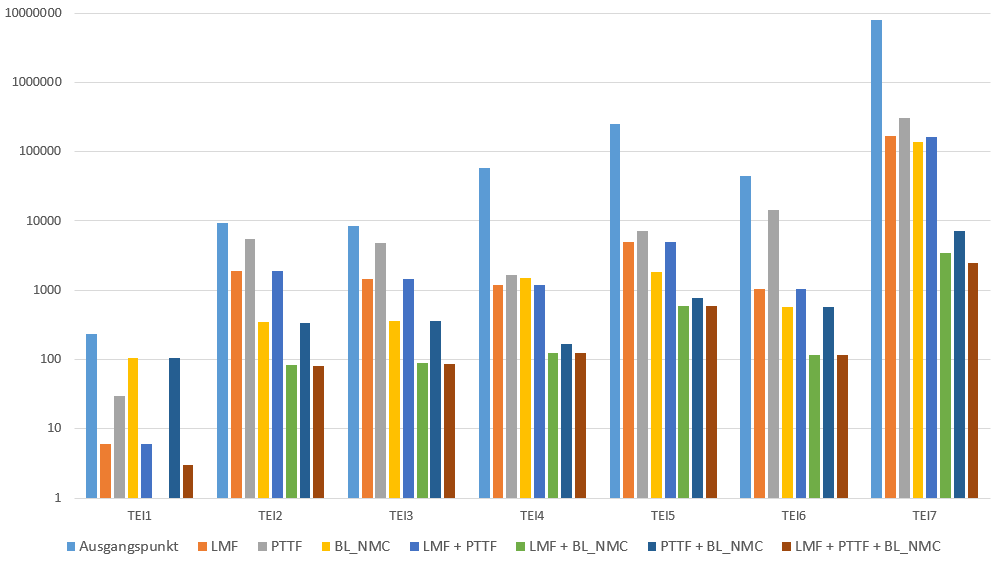
\includegraphics[width=\textwidth]{gegenueberstellung.png}
    \caption{Gegenüberstellung der Untersuchungsergebniss}
    \label{abb:gegenueberstellung}
\end{sidewaysfigure}



\backmatter{6}

\begin{appendix}
\section{Beispiel-Implementierungen f�r die Matcher}\label{matcherExamples}
Um die Beispiel-Implementierungen der Matcher nachvollziehen zu k�nnen, ist es notwendig die Implementierung der darin verwendeten Klassen aufzuzeigen. Daher sind diese in \lstsrefs{LST_superclass_impl}{LST_SuperWrapperReturnSubWrapperParamClass_impl} aufgef�hrt. Dabei handelt es sich zum einen um die Implementierungen der Klassen, die in den Szenarien der Abschnitte \ref{exactTypeMatcher} - \ref{structTypeMatcher} beschrieben wurden. Zum anderen handelt es sich um Implementierung weiterer Klassen, die in Szenarien verwendet werden, welche in den folgenden Abschnitten aufgef�hrt werden. Um einen �berblick zu gew�hrleisten, zeigt \abbref{cd_alltypes} alle Typen auf, die in den Szenarien verwendet werden.

\myBigFigure{cd_alltypes}{Alle Typen/Klassen, die in Matcher-Szenarien verwendet werden}{cd_alltypes}

\begin{lstlisting}[{caption = Implemetierung: SuperClass
},{label = LST_superclass_impl}]
public class SuperClass {

  private String string;

  public SuperClass( String string ) {
    this.string = string;
  }

  public String getString() {
    return string;
  }
}
\end{lstlisting}


\begin{lstlisting}[{caption = Implemetierung: SubClass
},{label = LST_subclass_impl}]
public class SubClass extends SuperClass {

  public SubClass( String string ) {
    super( "Sub" + string );
  }

  public String getStringWithoutPrefix() {
    return getString().substring( 3 );
  }
}
\end{lstlisting}




\begin{lstlisting}[{caption = Implemetierung: SubWrapper
},{label = LST_subwrapper_impl}]
public class SubWrapper {

  private SubClass wrapped;

  public SubWrapper( String string ) {
    this.wrapped = new SubClass( string );
  }

  @Override
  public String toString() {
    return "WRAPPED_" + this.wrapped.getStringWithoutPrefix();
  }

  public String toStringWithPrefix() {
    return "WRAPPED_" + this.wrapped.getString();
  }
}
\end{lstlisting}





\begin{lstlisting}[{caption = Implemetierung: SuperWrapperReturnSubWrapperParamClass
},{label = LST_SuperWrapperReturnSubWrapperParamClass_impl}]
public class SuperWrapperReturnSubWrapperParamClass {

  public SuperWrapper addHello( SubWrapper a ) {
    return new SuperWrapper( a.toString() + "hello" );
  }

  public SuperWrapper add( SubWrapper a, SubWrapper b ) {
    return new SuperWrapper( a.toString() + b.toString() );
  }
}
\end{lstlisting}

\subsection{Beispiel f�r den ExactTypeMatcher}\label{exactMatcherExample}
In \lstref{LST_exactTypeMatcher_matching} ist die Implementierung eines JUnit-Tests aufgef�hrt, in dem das Matching �ber den ExactTypeMatcher f�r unterschiedliche Source- und Target-Typen nachgewiesen werden soll. Die Test-Methode match enth�lt dabei die Aufrufe, bei denen das Matching festgestellt werden kann. Dementsprechend enth�lt die Test-Methode noMatch die Aufrufe, bei denen das Matching fehlschl�gt.\\\\
\lstref{LST_exactTypeMatcher_conversion} enth�lt die Implementierung f�r einen JUnit-Test, in dem die Konvertierung, die durch den ExactTypeMatcher beschrieben wird, nachgewiesen wird. Hierbei wird von dem Szenario aus \ref{exactTypeMatcher} ausgegangen.
\begin{lstlisting}[{caption = ExactTypeMatcher Matching Test
},{label = LST_exactTypeMatcher_matching}]
public class ExactTypeMatcher_MatcherTest {

  @Test
  public void match() {
    ExactTypeMatcher matcher = new ExactTypeMatcher();
    assertTrue( matcher.matchesType( String.class, String.class ) );
    assertTrue( matcher.matchesType( int.class, int.class ) );
    assertTrue( matcher.matchesType( Object.class, Object.class ) );
    assertTrue( matcher.matchesType( SuperClass.class, SuperClass.class ) );
  }

  @Test
  public void noMatch() {
    ExactTypeMatcher matcher = new ExactTypeMatcher();
    assertFalse( matcher.matchesType( String.class, int.class ) );
    assertFalse( matcher.matchesType( int.class, Object.class ) );
    assertFalse( matcher.matchesType( Object.class, String.class ) );
    assertFalse( matcher.matchesType( SuperClass.class, SubClass.class ) );
  }
}
\end{lstlisting}

\begin{lstlisting}[{caption = ExactTypeMatcher Konvertierung Test
},{label = LST_exactTypeMatcher_conversion}]
public class ExactTypeMatcher_ConversionTest {

  @Test
  public void convertString() {
    SuperClass target = new SuperClass( "A" );
    Collection<ModuleMatchingInfo> matchingInfos = new ExactTypeMatcher().calculateTypeMatchingInfos( SuperClass.class,
        SuperClass.class );
    
    ModuleMatchingInfo moduleMatchingInfo = matchingInfos.iterator().next();

    ProxyFactory<SuperClass> proxyFactory = moduleMatchingInfo.getConverterCreator()
        .createProxyFactory( SuperClass.class );
    Collection<MethodMatchingInfo> methodMatchingInfos = moduleMatchingInfo.getMethodMatchingInfos();

    SuperClass source = proxyFactory.createProxy( target, methodMatchingInfos );

    assertTrue( source.getString().equals( "A" ) );
  }
}
\end{lstlisting}

\subsection{Beispiel f�r den GenTypeMatcher}\label{genMatcherExample}
Der GenTypeMatcher und der SpecTypeMatcher wurden gemeinsam implementiert. Daher wird in den folgenden Beispielen jeweils ein Matcher aus der Klasse GenSpecTypeMatcher erzeugt. Die weitere Verwendung den Matchers bezieht sich in diesen Beispielen aber auf die Definition des GenTypeMatchers aus \ref{genTypeMatcher}.\\\\
In \lstref{LST_genTypeMatcher_matching} ist die Implementierung eines JUnit-Tests aufgef�hrt, in dem das Matching �ber den GenTypeMatcher f�r unterschiedliche Source- und Target-Typen nachgewiesen werden soll. Die Test-Methode match enth�lt dabei die Aufrufe, bei denen das Matching festgestellt werden kann. Dementsprechend enth�lt die Test-Methode noMatch die Aufrufe, bei denen das Matching fehlschl�gt.\\\\
\lstref{LST_genTypeMatcher_conversion} enth�lt die Implementierung f�r einen JUnit-Test, in dem die Konvertierung, die durch den GenTypeMatcher beschrieben wird, nachgewiesen wird. Hierbei wird von dem Szenario aus \ref{genTypeMatcher} ausgegangen.
\begin{lstlisting}[{caption = GenTypeMatcher Matching Test
},{label = LST_genTypeMatcher_matching}]
public class GenSpecTypeMatcher_Gen_MatcherTest {

  @Test
  public void match() {
    GenSpecTypeMatcher matcher = new GenSpecTypeMatcher();
    assertTrue( matcher.matchesType( Object.class, String.class ) );
    assertTrue( matcher.matchesType( SuperClass.class, SubClass.class ) );
    assertTrue( matcher.matchesType( Number.class, Integer.class ) );
  }

  @Test
  public void noMatch() {
    GenSpecTypeMatcher matcher = new GenSpecTypeMatcher();
    assertFalse( matcher.matchesType( int.class, String.class ) );
  }
}
\end{lstlisting}
\begin{lstlisting}[{caption = GenTypeMatcher Konvertierung Test
},{label = LST_genTypeMatcher_conversion}]
public class GenSpecTypeMatcher_Gen_ConversionTest {

  @Test
  public void convertSpec2Gen() {
   SubClass target = new SubClass( "A" );
    Collection<ModuleMatchingInfo> matchingInfos = new GenSpecTypeMatcher().calculateTypeMatchingInfos(
        SuperClass.class, SubClass.class );
    
    ModuleMatchingInfo moduleMatchingInfo = matchingInfos.iterator().next();

    ProxyFactory<SuperClass> proxyFactory = moduleMatchingInfo.getConverterCreator()
        .createProxyFactory( SuperClass.class );
    Collection<MethodMatchingInfo> methodMatchingInfos = moduleMatchingInfo.getMethodMatchingInfos();

    SuperClass source = proxyFactory.createProxy( target, methodMatchingInfos );

    assertTrue( source.getString().equals( "SubA" ) );
  }
}
\end{lstlisting}


\subsection{Beispiel f�r den SpecTypeMatcher}\label{specMatcherExample}
Wie in \ref{genTypeMatcher} bereits erw�hnt wurde der GenTypeMatcher gemeinsam mit dem SpecTypeMatcher implementiert. Daher wird in den folgenden Beispielen jeweils ein Matcher aus der Klasse GenSpecTypeMatcher erzeugt. Die weitere Verwendung den Matchers bezieht sich in diesen Beispielen aber auf die Definition des SpecTypeMatcher aus \ref{specTypeMatcher}.\\\\
In \lstref{LST_specTypeMatcher_matching} ist die Implementierung eines JUnit-Tests aufgef�hrt, in dem das Matching �ber den GenTypeMatcher f�r unterschiedliche Source- und Target-Typen nachgewiesen werden soll. Die Test-Methode match enth�lt dabei die Aufrufe, bei denen das Matching festgestellt werden kann. Dementsprechend enth�lt die Test-Methode noMatch die Aufrufe, bei denen das Matching fehlschl�gt.\\\\
\lstref{LST_specTypeMatcher_conversion} enth�lt die Implementierung f�r einen JUnit-Test, in dem die Konvertierung, die durch den SpecTypeMatcher beschrieben wird, nachgewiesen wird. Hierbei wird von dem Szenario aus \ref{specTypeMatcher} ausgegangen. Die Test-Methode convertGen2Spec\_positivCall enth�lt den Aufruf der ersten Methoden aus dem Szenario (getString). Die Test-Methoden convertGen2Spec\_negativeCall beinhaltet den fehlschlagenden Aufruf der Methoden getStringWithoutPrefix.
\begin{lstlisting}[{caption = SpecTypeMatcher Matching Test
},{label = LST_specTypeMatcher_matching}]
public class GenSpecTypeMatcher_Spec_MatcherTest {

  @Test
  public void match() {
    GenSpecTypeMatcher matcher = new GenSpecTypeMatcher();
    assertTrue( matcher.matchesType( String.class, Object.class ) );
    assertTrue( matcher.matchesType( SubClass.class, SuperClass.class ) );
    assertTrue( matcher.matchesType( Integer.class, Number.class ) );
  }

  @Test
  public void noMatch() {
    GenSpecTypeMatcher matcher = new GenSpecTypeMatcher();
    assertFalse( matcher.matchesType( int.class, String.class ) );
  }
}
\end{lstlisting}
\begin{lstlisting}[{caption = SpecTypeMatcher Konvertierung Test
},{label = LST_specTypeMatcher_conversion}]
public class GenSpecTypeMatcher_Spec_ConversionTest {

  @Test
  public void convertGen2Spec_positivCall() {
    SuperClass offeredComponent = new SuperClass( "A" );
    Collection<ModuleMatchingInfo> matchingInfos = new GenSpecTypeMatcher().calculateTypeMatchingInfos(
        SubClass.class, SuperClass.class );
    
    ModuleMatchingInfo moduleMatchingInfo = matchingInfos.iterator().next();

    ProxyFactory<SubClass> proxyFactory = moduleMatchingInfo.getConverterCreator().createProxyFactory( SubClass.class );
    Collection<MethodMatchingInfo> methodMatchingInfos = moduleMatchingInfo.getMethodMatchingInfos();

    SubClass proxy = proxyFactory.createProxy( offeredComponent, methodMatchingInfos );

    assertTrue( proxy.getString().equals( "A" ) );
  }

  @Test( expected = SigMaGlueException.class )
  public void convertGen2Spec_negativeCall() {
    SuperClass offeredComponent = new SuperClass( "A" );
    Collection<ModuleMatchingInfo> matchingInfos = new GenSpecTypeMatcher().calculateTypeMatchingInfos(
        SubClass.class, SuperClass.class );
    
    ModuleMatchingInfo moduleMatchingInfo = matchingInfos.iterator().next();

    ProxyFactory<SubClass> proxyFactory = moduleMatchingInfo.getConverterCreator().createProxyFactory( SubClass.class );
    Collection<MethodMatchingInfo> methodMatchingInfos = moduleMatchingInfo.getMethodMatchingInfos();

    SubClass proxy = proxyFactory.createProxy( offeredComponent, methodMatchingInfos );

    assertTrue( proxy.getString().equals( "A" ) );

    proxy.getStringWithoutPrefix();
  }
}
\end{lstlisting}



\subsection{Beispiel f�r den WrappedTypeMatcher}\label{wrappedMatcherExample}
Der WrappedTypeMatcher und der WrapperTypeMatcher wurden gemeinsam implementiert. Daher wird in den folgenden Beispielen jeweils ein Matcher aus der Klasse WrappedTypeMatcher erzeugt. Die weitere Verwendung den Matchers bezieht sich in diesen Beispielen aber auf die Definition des WrappedTypeMatcher aus \ref{wrappedTypeMatcher}.\\\\
In \lstref{LST_wrappedTypeMatcher_matching} ist die Implementierung eines JUnit-Tests aufgef�hrt, in dem das Matching �ber den WrappedTypeMatcher f�r unterschiedliche Source- und Target-Typen nachgewiesen werden soll. Die Test-Methoden mit dem Pr�fix match enthalten dabei die Aufrufe, bei denen das Matching festgestellt werden kann. Dementsprechend enth�lt die Test-Methode noMatch die Aufrufe, bei denen das Matching fehlschl�gt.\\\\
\lstref{LST_wrappedTypeMatcher_conversion} enth�lt die Implementierung f�r einen JUnit-Test, in dem die Konvertierung, die durch den WrappedTypeMatcher beschrieben wird, nachgewiesen wird. In der Test-Methode convertSubWrapper2SubClass wird von dem Szenario aus \ref{wrappedTypeMatcher} ausgegangen. Die anderen Test-Methoden stellen weitere Szenarien dar, die in den folgenden Unterabschnitten beschrieben werden.
\begin{lstlisting}[{caption = WrappedTypeMatcher Matching Test
},{label = LST_wrappedTypeMatcher_matching}]
public class WrappedTypeMatcher_Wrapped_MatcherTest {

  private WrappedTypeMatcher matcher = new WrappedTypeMatcher(
      MatcherCombiner.combine( new ExactTypeMatcher(), new GenSpecTypeMatcher() ) );

  @Test
  public void match() {
    assertTrue( matcher.matchesType( boolean.class, Boolean.class ) );
    assertTrue( matcher.matchesType( int.class, Integer.class ) );
  }

  @Test
  public void match_wrapped_exact() {
    assertTrue( matcher.matchesType( SubClass.class, SubWrapper.class ) );
  }

  @Test
  public void match_wrapped_spec() {
    assertTrue( matcher.matchesType( SubClass.class, SuperWrapper.class ) );
  }

  @Test
  public void match_wrapped_gen() {
    assertTrue( matcher.matchesType( SuperClass.class, SubWrapper.class ) );
  }

  @Test
  public void noMatch() {
    assertFalse( matcher.matchesType( String.class, String.class ) );
  }
}
\end{lstlisting}
\begin{lstlisting}[{caption = WrappedTypeMatcher Konvertierung Test
},{label = LST_wrappedTypeMatcher_conversion}]
public class WrappedTypeMatcher_Wrapped_ConversionTest {

  private WrappedTypeMatcher matcher = new WrappedTypeMatcher(
      MatcherCombiner.combine( new ExactTypeMatcher(), new GenSpecTypeMatcher() ) );

  @Test
  public void convertSubWrapper2SubClass() {
    SubWrapper offeredComponent = new SubWrapper( "A" );
    Collection<ModuleMatchingInfo> matchingInfos = matcher.calculateTypeMatchingInfos(
        SubClass.class, SubWrapper.class );
  
    ModuleMatchingInfo moduleMatchingInfo = matchingInfos.iterator().next();

    ProxyFactory<SubClass> proxyFactory = moduleMatchingInfo.getConverterCreator()
        .createProxyFactory( SubClass.class );
    Collection<MethodMatchingInfo> methodMatchingInfos = moduleMatchingInfo.getMethodMatchingInfos();

    SubClass proxy = proxyFactory.createProxy( offeredComponent, methodMatchingInfos );

    assertTrue( proxy.getString().equals( "SubA" ) );
    assertTrue( proxy.getStringWithoutPrefix().equals( "A" ) );
  }

  @Test
  public void convertSuperWrapper2SubClass_positiveCall() {
    SuperWrapper offeredComponent = new SuperWrapper( "A" );
    Collection<ModuleMatchingInfo> matchingInfos = matcher.calculateTypeMatchingInfos(
        SubClass.class, SuperWrapper.class );
  
    ModuleMatchingInfo moduleMatchingInfo = matchingInfos.iterator().next();

    ProxyFactory<SubClass> proxyFactory = moduleMatchingInfo.getConverterCreator()
        .createProxyFactory( SubClass.class );
    Collection<MethodMatchingInfo> methodMatchingInfos = moduleMatchingInfo.getMethodMatchingInfos();

    SubClass proxy = proxyFactory.createProxy( offeredComponent, methodMatchingInfos );

    assertTrue( proxy.getString().equals( "A" ) );
  }

  @Test( expected = SigMaGlueException.class )
  public void convertSuperWrapper2SubClass_negativeCall() {
    SuperWrapper offeredComponent = new SuperWrapper( "A" );
    Collection<ModuleMatchingInfo> matchingInfos = matcher.calculateTypeMatchingInfos(
        SubClass.class, SuperWrapper.class );
  
    ModuleMatchingInfo moduleMatchingInfo = matchingInfos.iterator().next();

    ProxyFactory<SubClass> proxyFactory = moduleMatchingInfo.getConverterCreator()
        .createProxyFactory( SubClass.class );
    Collection<MethodMatchingInfo> methodMatchingInfos = moduleMatchingInfo.getMethodMatchingInfos();

    SubClass proxy = proxyFactory.createProxy( offeredComponent, methodMatchingInfos );
    proxy.getStringWithoutPrefix();
  }

  @Test
  public void convertSubWrapper2SuperClass() {
    SubWrapper offeredComponent = new SubWrapper( "A" );
    Collection<ModuleMatchingInfo> matchingInfos = matcher.calculateTypeMatchingInfos(
        SuperClass.class, SubWrapper.class );
   
    ModuleMatchingInfo moduleMatchingInfo = matchingInfos.iterator().next();

    ProxyFactory<SuperClass> proxyFactory = moduleMatchingInfo.getConverterCreator()
        .createProxyFactory( SuperClass.class );
    Collection<MethodMatchingInfo> methodMatchingInfos = moduleMatchingInfo.getMethodMatchingInfos();

    SuperClass proxy = proxyFactory.createProxy( offeredComponent, methodMatchingInfos );

    assertTrue( proxy.getString().equals( "SubA" ) );
  }
}
\end{lstlisting}





\subsection{Beispiel f�r den WrapperTypeMatcher}\label{wrapperMatcherExample}
Wie bereits im vorherigen Abschnitt erw�hnt wurden der WrappedTypeMatcher und der WrapperTypeMatcher gemeinsam implementiert. Daher wird in den folgenden Beispielen jeweils ein Matcher aus der Klasse WrappedTypeMatcher erzeugt. Die weitere Verwendung den Matchers bezieht sich in diesen Beispielen aber auf die Definition des WrapperTypeMatcher aus \ref{wrapperTypeMatcher}.\\\\
In \lstref{LST_wrapperTypeMatcher_matching} ist die Implementierung eines JUnit-Tests aufgef�hrt, in dem das Matching �ber den WrapperTypeMatcher f�r unterschiedliche Source- und Target-Typen nachgewiesen werden soll. Die Test-Methoden mit dem Pr�fix match enthalten dabei die Aufrufe, bei denen das Matching festgestellt werden kann. Dementsprechend enth�lt die Test-Methode noMatch die Aufrufe, bei denen das Matching fehlschl�gt.\\\\
\lstref{LST_wrapperTypeMatcher_conversion} enth�lt die Implementierung f�r einen JUnit-Test, in dem die Konvertierung, die durch den WrapperTypeMatcher beschrieben wird, nachgewiesen wird. In der Test-Methode convertSubClass2SubWrapper wird von dem Szenario aus \ref{wrapperTypeMatcher} ausgegangen. Die anderen Test-Methoden stellen weitere Szenarien dar, die in den folgenden Unterabschnitten beschrieben werden.
\begin{lstlisting}[{caption = WrapperTypeMatcher Matching Test
},{label = LST_wrapperTypeMatcher_matching}]
public class WrappedTypeMatcher_Wrapper_MatcherTest {

  private WrappedTypeMatcher matcher = new WrappedTypeMatcher(
      MatcherCombiner.combine( new ExactTypeMatcher(), new GenSpecTypeMatcher() ) );

  @Test
  public void match() {
    assertTrue( matcher.matchesType( Boolean.class, boolean.class ) );
    assertTrue( matcher.matchesType( Integer.class, int.class ) );
  }

  @Test
  public void match_wrapped_exact() {
    assertTrue( matcher.matchesType( SubWrapper.class, SubClass.class ) );
  }

  @Test
  public void match_wrapped_spec() {
    assertTrue( matcher.matchesType( SuperWrapper.class, SubClass.class ) );
  }

  @Test
  public void match_wrapped_gen() {
    assertTrue( matcher.matchesType( SubWrapper.class, SuperClass.class ) );
  }

  @Test
  public void noMatch() {
    assertFalse( matcher.matchesType( String.class, String.class ) );
  }
}
\end{lstlisting}
\begin{lstlisting}[{caption = WrapperTypeMatcher Konvertierung Test
},{label = LST_wrapperTypeMatcher_conversion}]
public class WrappedTypeMatcher_Wrapper_ConversionTest {

  private WrappedTypeMatcher matcher = new WrappedTypeMatcher(
      MatcherCombiner.combine( new ExactTypeMatcher(), new GenSpecTypeMatcher() ) );

  @Test
  public void convertSubClass2SubWrapper() {
    SubClass offeredComponent = new SubClass( "A" );
    Collection<ModuleMatchingInfo> matchingInfos = matcher.calculateTypeMatchingInfos(
        SubWrapper.class, SubClass.class );

    ModuleMatchingInfo moduleMatchingInfo = matchingInfos.iterator().next();

    ProxyFactory<SubWrapper> proxyFactory = moduleMatchingInfo.getConverterCreator()
        .createProxyFactory( SubWrapper.class );
    Collection<MethodMatchingInfo> methodMatchingInfos = moduleMatchingInfo.getMethodMatchingInfos();

    SubWrapper proxy = proxyFactory.createProxy( offeredComponent, methodMatchingInfos );

    assertTrue( proxy.toString().equals( "WRAPPED_A" ) );
    assertTrue( proxy.toStringWithPrefix().equals( "WRAPPED_SubA" ) );
  }

  @Test
  public void convertSuperWrapper2SubClass() {
    SubClass offeredComponent = new SubClass( "A" );
    Collection<ModuleMatchingInfo> matchingInfos = matcher.calculateTypeMatchingInfos(
        SuperWrapper.class, SubClass.class );

    ModuleMatchingInfo moduleMatchingInfo = matchingInfos.iterator().next();

    ProxyFactory<SuperWrapper> proxyFactory = moduleMatchingInfo.getConverterCreator()
        .createProxyFactory( SuperWrapper.class );
    Collection<MethodMatchingInfo> methodMatchingInfos = moduleMatchingInfo.getMethodMatchingInfos();

    SuperWrapper proxy = proxyFactory.createProxy( offeredComponent, methodMatchingInfos );

    assertTrue( proxy.toString().equals( "WRAPPED_SubA" ) );
    assertFalse( proxy.hashCode() == offeredComponent.hashCode() );
  }

  @Test
  public void convertSubWrapper2SuperClass_positiveCall() {
    SuperClass offeredComponent = new SuperClass( "A" );
    Collection<ModuleMatchingInfo> matchingInfos = matcher.calculateTypeMatchingInfos(
        SubWrapper.class, SuperClass.class );

    ModuleMatchingInfo moduleMatchingInfo = matchingInfos.iterator().next();

    ProxyFactory<SubWrapper> proxyFactory = moduleMatchingInfo.getConverterCreator()
        .createProxyFactory( SubWrapper.class );
    Collection<MethodMatchingInfo> methodMatchingInfos = moduleMatchingInfo.getMethodMatchingInfos();

    SubWrapper proxy = proxyFactory.createProxy( offeredComponent, methodMatchingInfos );

    assertTrue( proxy.toStringWithPrefix().equals( "WRAPPED_A" ) );
    assertFalse( proxy.hashCode() == offeredComponent.hashCode() );
  }

  @Test( expected = SigMaGlueException.class )
  public void convertSubWrapper2SuperClass_negativeCall() {
    SuperClass offeredComponent = new SuperClass( "A" );
    Collection<ModuleMatchingInfo> matchingInfos = matcher.calculateTypeMatchingInfos(
        SubWrapper.class, SuperClass.class );
    // Der WrappedTypeMatcher erzeugt nur eine ModuleMatchingInfo (kein rekursives Matching)
    ModuleMatchingInfo moduleMatchingInfo = matchingInfos.iterator().next();

    ProxyFactory<SubWrapper> proxyFactory = moduleMatchingInfo.getConverterCreator()
        .createProxyFactory( SubWrapper.class );
    Collection<MethodMatchingInfo> methodMatchingInfos = moduleMatchingInfo.getMethodMatchingInfos();

    SubWrapper proxy = proxyFactory.createProxy( offeredComponent, methodMatchingInfos );

    proxy.toString().equals( "WRAPPED_A" );
  }
}

\end{lstlisting}



\subsection{Beispiel f�r den StructuralTypeMatcher}\label{structMatcherExample}
In \lstref{LST_structTypeMatcher_matching} ist die Implementierung eines JUnit-Tests aufgef�hrt, in dem das Matching �ber den StructuralTypeMatcher f�r unterschiedliche Source- und Target-Typen nachgewiesen werden soll. Alle Test-Methoden enthalten Aufrufe, bei denen das Matching festgestellt werden kann. Die Test-Methode match\_genReturn\_specParam bezieht sich auf das Szenario aus \ref{wrapperTypeMatcher}.   Da es f�r jedes Paar von Source- und Target-Typ mehrere M�glichkeiten zur Feststellung der strukturellen Gleichheit gibt, wird die Evaluation der Testf�lle in einer Schleife �ber diese M�glichkeiten durchgef�hrt.\\\\
\lstref{LST_structTypeMatcher_conversion} enth�lt die Implementierung f�r einen JUnit-Test, in dem die Konvertierung, die durch den StructTypeMatcher beschrieben wird, nachgewiesen wird. Die Test-Methode convert\_genReturn\_specParam bezieht sich dabei auf das Szenario aus \ref{structTypeMatcher}. Die anderen Test-Methoden stellen weitere Szenarien dar, die in den folgenden Unterabschnitten beschrieben werden.\\\\
In beiden F�llen wurde von einem StructuralTypeMatcher ausgegangen, der als internen Type-Matcher eine Kombination aus den zuvor genannten Matchern verwendet.
\begin{lstlisting}[{caption = StructTypeMatcher Matching Test
},{label = LST_structTypeMatcher_matching}]
public class StructuralTypeMatcher_MatcherTest {

  private StructuralTypeMatcher matcher = new StructuralTypeMatcher(
      MatcherCombiner.combine( new ExactTypeMatcher(), new GenSpecTypeMatcher(),
          new WrappedTypeMatcher( MatcherCombiner.combine( new ExactTypeMatcher(), new GenSpecTypeMatcher() ) ) ) );

  @Test
  public void match_exactReturn_exactParam() {
    assertTrue( matcher.matchesType( SubReturnSubParamClass1.class, SubReturnSubParamClass2.class ) );
  }

  @Test
  public void match_exactReturn_genParam() {
    assertTrue( matcher.matchesType( SubReturnSuperParamClass.class, SubReturnSubParamClass1.class ) );
  }

  @Test
  public void match_exactReturn_specParam() {
    assertTrue( matcher.matchesType( SubReturnSubParamClass1.class, SubReturnSuperParamClass.class ) );
  }

  @Test
  public void match_genReturn_specParam() {
    assertTrue( matcher.matchesType( SuperReturnSubParamClass.class, SubReturnSuperParamClass.class ) );
  }

  @Test
  public void match_specReturn_genParam() {
    assertTrue( matcher.matchesType( SubReturnSuperParamClass.class, SuperReturnSubParamClass.class ) );
  }

  @Test
  public void match_specReturn_wrapperGenParam() {
    assertTrue( matcher.matchesType( SubReturnSuperWrapperParamClass.class, SuperReturnSubParamClass.class ) );
  }

  @Test
  public void match_wrapperGenReturn_specParam() {
    assertTrue( matcher.matchesType( SuperWrapperReturnSubParamClass.class, SubReturnSuperParamClass.class ) );
  }

  @Test
  public void match_wrapperGenReturn_wrapperSpecParam() {
    assertTrue( matcher.matchesType( SuperWrapperReturnSubWrapperParamClass.class, SubReturnSuperParamClass.class ) );
  }

  @Test
  public void match_wrapperSpecReturn_wrapperExactParam() {
    assertTrue( matcher.matchesType( SubWrapperReturnSubParamClass.class, SuperReturnSubParamClass.class ) );
  }
}
\end{lstlisting}

\begin{lstlisting}[{caption = StructuralTypeMatcher Konvertierung Test
},{label = LST_structTypeMatcher_conversion}]
public class StructuralTypeMatcher_ConversionTest {

  private StructuralTypeMatcher matcher = new StructuralTypeMatcher(
      MatcherCombiner.combine( new ExactTypeMatcher(), new GenSpecTypeMatcher(),
          new WrappedTypeMatcher( MatcherCombiner.combine( new ExactTypeMatcher(), new GenSpecTypeMatcher() ) ) ) );

  @Test
  public void convert_exactReturn_exactParam() {
    SubReturnSubParamClass2 offeredComponent = new SubReturnSubParamClass2();
    Collection<ModuleMatchingInfo> matchingInfos = matcher.calculateTypeMatchingInfos( SubReturnSubParamClass1.class,
        SubReturnSubParamClass2.class );

    for ( ModuleMatchingInfo moduleMatchingInfo : matchingInfos ) {
      ProxyFactory<SubReturnSubParamClass1> proxyFactory = moduleMatchingInfo.getConverterCreator()
          .createProxyFactory( SubReturnSubParamClass1.class );
      Collection<MethodMatchingInfo> methodMatchingInfos = moduleMatchingInfo.getMethodMatchingInfos();

      SubReturnSubParamClass1 proxy = proxyFactory.createProxy( offeredComponent, methodMatchingInfos );

      SubClass param1 = new SubClass( "A" );
      SubClass param2 = new SubClass( "B" );
      assertTrue( proxy.addHello( param1 ).getString().equals( "SubSubAhello" ) );
      assertTrue( proxy.addHello( param1 ).getStringWithoutPrefix().equals( "SubAhello" ) );
      assertTrue( proxy.add( param1, param2 ).getString().equals( "SubSubASubB" ) );
      assertTrue( proxy.add( param1, param2 ).getStringWithoutPrefix().equals( "SubASubB" ) );
    }
  }

  @Test
  public void convert_exactReturn_genParam() {
    SubReturnSubParamClass1 offeredComponent = new SubReturnSubParamClass1();
    Collection<ModuleMatchingInfo> matchingInfos = matcher.calculateTypeMatchingInfos( SubReturnSuperParamClass.class,
        SubReturnSubParamClass1.class );
    for ( ModuleMatchingInfo moduleMatchingInfo : matchingInfos ) {
      ProxyFactory<SubReturnSuperParamClass> proxyFactory = moduleMatchingInfo.getConverterCreator()
          .createProxyFactory( SubReturnSuperParamClass.class );
      Collection<MethodMatchingInfo> methodMatchingInfos = moduleMatchingInfo.getMethodMatchingInfos();

      SubReturnSuperParamClass proxy = proxyFactory.createProxy( offeredComponent, methodMatchingInfos );

      SuperClass param1 = new SuperClass( "A" );
      SuperClass param2 = new SuperClass( "B" );
      assertTrue( proxy.addHello( param1 ).getString().equals( "SubAhello" ) );
      assertTrue( proxy.addHello( param1 ).getStringWithoutPrefix().equals( "Ahello" ) );
      assertTrue( proxy.add( param1, param2 ).getString().equals( "SubAB" ) );
      assertTrue( proxy.add( param1, param2 ).getStringWithoutPrefix().equals( "AB" ) );
    }
  }

  @Test
  public void convert_exactReturn_specParam() {
    SubReturnSuperParamClass offeredComponent = new SubReturnSuperParamClass();
    Collection<ModuleMatchingInfo> matchingInfos = matcher.calculateTypeMatchingInfos( SubReturnSubParamClass1.class,
        SubReturnSuperParamClass.class );
    for ( ModuleMatchingInfo moduleMatchingInfo : matchingInfos ) {
      ProxyFactory<SubReturnSubParamClass1> proxyFactory = moduleMatchingInfo.getConverterCreator()
          .createProxyFactory( SubReturnSubParamClass1.class );
      Collection<MethodMatchingInfo> methodMatchingInfos = moduleMatchingInfo.getMethodMatchingInfos();

      SubReturnSubParamClass1 proxy = proxyFactory.createProxy( offeredComponent, methodMatchingInfos );

      SubClass param1 = new SubClass( "A" );
      SubClass param2 = new SubClass( "B" );
      assertTrue( proxy.addHello( param1 ).getString().equals( "SubSubAhello" ) );
      assertTrue( proxy.addHello( param1 ).getStringWithoutPrefix().equals( "SubAhello" ) );
      assertTrue( proxy.add( param1, param2 ).getString().equals( "SubSubASubB" ) );
      assertTrue( proxy.add( param1, param2 ).getStringWithoutPrefix().equals( "SubASubB" ) );
    }
  }

  @Test
  public void convert_genReturn_specParam() {
    SubReturnSuperParamClass offeredComponent = new SubReturnSuperParamClass();
    Collection<ModuleMatchingInfo> matchingInfos = matcher.calculateTypeMatchingInfos( SuperReturnSubParamClass.class,
        SubReturnSuperParamClass.class );
    for ( ModuleMatchingInfo moduleMatchingInfo : matchingInfos ) {
      ProxyFactory<SuperReturnSubParamClass> proxyFactory = moduleMatchingInfo.getConverterCreator()
          .createProxyFactory( SuperReturnSubParamClass.class );
      Collection<MethodMatchingInfo> methodMatchingInfos = moduleMatchingInfo.getMethodMatchingInfos();

      SuperReturnSubParamClass proxy = proxyFactory.createProxy( offeredComponent, methodMatchingInfos );

      SubClass param1 = new SubClass( "A" );
      SubClass param2 = new SubClass( "B" );
      assertTrue( proxy.helloAdd( param1 ).getString().equals( "helloSubA" ) );
      assertTrue( proxy.addParams( param1, param2 ).getString().equals( "SubASubB" ) );
    }
  }

  @Test
  public void convert_specReturn_genParam() {
    SuperReturnSubParamClass offeredComponent = new SuperReturnSubParamClass();
    Collection<ModuleMatchingInfo> matchingInfos = matcher.calculateTypeMatchingInfos( SubReturnSuperParamClass.class,
        SuperReturnSubParamClass.class );
    for ( ModuleMatchingInfo moduleMatchingInfo : matchingInfos ) {
      ProxyFactory<SubReturnSuperParamClass> proxyFactory = moduleMatchingInfo.getConverterCreator()
          .createProxyFactory( SubReturnSuperParamClass.class );
      Collection<MethodMatchingInfo> methodMatchingInfos = moduleMatchingInfo.getMethodMatchingInfos();

      SubReturnSuperParamClass proxy = proxyFactory.createProxy( offeredComponent, methodMatchingInfos );

      SuperClass param1 = new SuperClass( "A" );
      SuperClass param2 = new SuperClass( "B" );
      assertTrue( proxy.addHello( param1 ).getString().equals( "SubAhello" ) );
      assertTrue( proxy.addHello( param1 ).getStringWithoutPrefix().equals( "Ahello" ) );
      assertTrue( proxy.add( param1, param2 ).getString().equals( "SubAB" ) );
      assertTrue( proxy.add( param1, param2 ).getStringWithoutPrefix().equals( "AB" ) );
    }

  }

  @Test
  public void convert_specReturn_wrapperGenParam() {
    SuperReturnSubParamClass offeredComponent = new SuperReturnSubParamClass();
    Collection<ModuleMatchingInfo> matchingInfos = matcher.calculateTypeMatchingInfos(
        SubReturnSuperWrapperParamClass.class,
        SuperReturnSubParamClass.class );
    for ( ModuleMatchingInfo moduleMatchingInfo : matchingInfos ) {
      ProxyFactory<SubReturnSuperWrapperParamClass> proxyFactory = moduleMatchingInfo.getConverterCreator()
          .createProxyFactory( SubReturnSuperWrapperParamClass.class );
      Collection<MethodMatchingInfo> methodMatchingInfos = moduleMatchingInfo.getMethodMatchingInfos();

      SubReturnSuperWrapperParamClass proxy = proxyFactory.createProxy( offeredComponent, methodMatchingInfos );

      SuperWrapper param1 = new SuperWrapper( "A" );
      SuperWrapper param2 = new SuperWrapper( "B" );
      assertTrue( proxy.addHello( param1 ).getString().equals( "SubWRAPPED_Ahello" ) );
      assertTrue( proxy.addHello( param1 ).getStringWithoutPrefix().equals( "WRAPPED_Ahello" ) );
      assertTrue( proxy.add( param1, param2 ).getString().equals( "SubWRAPPED_AWRAPPED_B" ) );
      assertTrue( proxy.add( param1, param2 ).getStringWithoutPrefix().equals( "WRAPPED_AWRAPPED_B" ) );
    }
  }

  @Test
  public void convert_wrapperGenReturn_specParam() {
    SubReturnSuperParamClass offeredComponent = new SubReturnSuperParamClass();
    Collection<ModuleMatchingInfo> matchingInfos = matcher.calculateTypeMatchingInfos(
        SuperWrapperReturnSubParamClass.class,
        SubReturnSuperParamClass.class );
    for ( ModuleMatchingInfo moduleMatchingInfo : matchingInfos ) {
      ProxyFactory<SuperWrapperReturnSubParamClass> proxyFactory = moduleMatchingInfo.getConverterCreator()
          .createProxyFactory( SuperWrapperReturnSubParamClass.class );
      Collection<MethodMatchingInfo> methodMatchingInfos = moduleMatchingInfo.getMethodMatchingInfos();

      SuperWrapperReturnSubParamClass proxy = proxyFactory.createProxy( offeredComponent, methodMatchingInfos );

      SubClass param1 = new SubClass( "A" );
      SubClass param2 = new SubClass( "B" );
      assertTrue( proxy.addHello( param1 ).toString().equals( "WRAPPED_SubAhello" ) );
      assertTrue( proxy.add( param1, param2 ).toString().equals( "WRAPPED_SubASubB" ) );
    }
  }

  @Test
  public void convert_wrapperGenReturn_wrapperSpecParam() {
    SubReturnSuperParamClass offeredComponent = new SubReturnSuperParamClass();
    Collection<ModuleMatchingInfo> matchingInfos = matcher.calculateTypeMatchingInfos(
        SuperWrapperReturnSubWrapperParamClass.class,
        SubReturnSuperParamClass.class );
    for ( ModuleMatchingInfo moduleMatchingInfo : matchingInfos ) {
      ProxyFactory<SuperWrapperReturnSubWrapperParamClass> proxyFactory = moduleMatchingInfo.getConverterCreator()
          .createProxyFactory( SuperWrapperReturnSubWrapperParamClass.class );
      Collection<MethodMatchingInfo> methodMatchingInfos = moduleMatchingInfo.getMethodMatchingInfos();

      SuperWrapperReturnSubWrapperParamClass proxy = proxyFactory.createProxy( offeredComponent, methodMatchingInfos );

      SubWrapper param1 = new SubWrapper( "A" );
      SubWrapper param2 = new SubWrapper( "B" );
      assertTrue( proxy.addHello( param1 ).toString().equals( "WRAPPED_WRAPPED_Ahello" ) );
      assertTrue( proxy.add( param1, param2 ).toString().equals( "WRAPPED_WRAPPED_AWRAPPED_B" ) );
    }
  }

  @Test
  public void convert_wrapperSpecReturn_wrapperExactParam() {

    SuperReturnSubParamClass offeredComponent = new SuperReturnSubParamClass();
    Collection<ModuleMatchingInfo> matchingInfos = matcher.calculateTypeMatchingInfos(
        SubWrapperReturnSubParamClass.class,
        SuperReturnSubParamClass.class );
    for ( ModuleMatchingInfo moduleMatchingInfo : matchingInfos ) {
      ProxyFactory<SubWrapperReturnSubParamClass> proxyFactory = moduleMatchingInfo.getConverterCreator()
          .createProxyFactory( SubWrapperReturnSubParamClass.class );
      Collection<MethodMatchingInfo> methodMatchingInfos = moduleMatchingInfo.getMethodMatchingInfos();

      SubWrapperReturnSubParamClass proxy = proxyFactory.createProxy( offeredComponent, methodMatchingInfos );

      SubClass param1 = new SubClass( "A" );
      SubClass param2 = new SubClass( "B" );
      assertTrue( proxy.addHello( param1 ).toString().equals( "WRAPPED_SubAhello" ) );
      assertTrue( proxy.addHello( param1 ).toStringWithPrefix().equals( "WRAPPED_SubSubAhello" ) );
      assertTrue( proxy.add( param1, param2 ).toString().equals( "WRAPPED_SubASubB" ) );
      assertTrue( proxy.add( param1, param2 ).toStringWithPrefix().equals( "WRAPPED_SubSubASubB" ) );
    }
  }
}
\end{lstlisting}

%\include{AnhangB}
\end{appendix}


%\include{cd}


%\phantomsection
%\addcontentsline{toc}{chapter}{Literaturverzeichnis}
\bibliography{thesisbib}{}


\end{document}
